\documentclass{article}

% if you need to pass options to natbib, use, e.g.:
%     \PassOptionsToPackage{numbers, compress}{natbib}
% before loading neurips_2025

% The authors should use one of these tracks.
% Before accepting by the NeurIPS conference, select one of the options below.
% 0. "default" for submission
 \usepackage[preprint]{neurips_2025}
% the "default" option is equal to the "main" option, which is used for the Main Track with double-blind reviewing.
% 1. "main" option is used for the Main Track
%  \usepackage[main]{neurips_2025}
% 2. "position" option is used for the Position Paper Track
%  \usepackage[position]{neurips_2025}
% 3. "dandb" option is used for the Datasets & Benchmarks Track
 % \usepackage[dandb]{neurips_2025}
% 4. "creativeai" option is used for the Creative AI Track
%  \usepackage[creativeai]{neurips_2025}
% 5. "sglblindworkshop" option is used for the Workshop with single-blind reviewing
 % \usepackage[sglblindworkshop]{neurips_2025}
% 6. "dblblindworkshop" option is used for the Workshop with double-blind reviewing
%  \usepackage[dblblindworkshop]{neurips_2025}

% After being accepted, the authors should add "final" behind the track to compile a camera-ready version.
% 1. Main Track
 % \usepackage[main, final]{neurips_2025}
% 2. Position Paper Track
%  \usepackage[position, final]{neurips_2025}
% 3. Datasets & Benchmarks Track
 % \usepackage[dandb, final]{neurips_2025}
% 4. Creative AI Track
%  \usepackage[creativeai, final]{neurips_2025}
% 5. Workshop with single-blind reviewing
%  \usepackage[sglblindworkshop, final]{neurips_2025}
% 6. Workshop with double-blind reviewing
%  \usepackage[dblblindworkshop, final]{neurips_2025}
% Note. For the workshop paper template, both \title{} and \workshoptitle{} are required, with the former indicating the paper title shown in the title and the latter indicating the workshop title displayed in the footnote.
% For workshops (5., 6.), the authors should add the name of the workshop, "\workshoptitle" command is used to set the workshop title.
% \workshoptitle{WORKSHOP TITLE}

% "preprint" option is used for arXiv or other preprint submissions
 % \usepackage[preprint]{neurips_2025}

% to avoid loading the natbib package, add option nonatbib:
%    \usepackage[nonatbib]{neurips_2025}

\usepackage{siunitx}
\usepackage[utf8]{inputenc} % allow utf-8 input
\usepackage[T1]{fontenc}    % use 8-bit T1 fonts
\usepackage{hyperref}       % hyperlinks
\usepackage{url}            % simple URL typesetting
\usepackage{booktabs}       % professional-quality tables
\usepackage{amsfonts}       % blackboard math symbols
\usepackage{nicefrac}       % compact symbols for 1/2, etc.
\usepackage{microtype}      % microtypography
\usepackage{xcolor}         % colors



% Note. For the workshop paper template, both \title{} and \workshoptitle{} are required, with the former indicating the paper title shown in the title and the latter indicating the workshop title displayed in the footnote. 
\title{Deep Neural Networks with Gaussian Input}


% The \author macro works with any number of authors. There are two commands
% used to separate the names and addresses of multiple authors: \And and \AND.
%
% Using \And between authors leaves it to LaTeX to determine where to break the
% lines. Using \AND forces a line break at that point. So, if LaTeX puts 3 of 4
% authors names on the first line, and the last on the second line, try using
% \AND instead of \And before the third author name.


\author{%
  Simon Kuang and Xinfan Lin\thanks{\color{red} Use footnote for providing further information
    about author (webpage, alternative address)---\emph{not} for acknowledging
    funding agencies.} \\
  Department of Mechanical and Aerospace Engineering\\
  University of California, Davis\\
  Davis, CA 95616 \\
  \texttt{\{slku, lxflin\}@ucdavis.edu} \\
  % examples of more authors
  % \And
  % Coauthor \\
  % Affiliation \\
  % Address \\
  % \texttt{email} \\
  % \AND
  % Coauthor \\
  % Affiliation \\
  % Address \\
  % \texttt{email} \\
  % \And
  % Coauthor \\
  % Affiliation \\
  % Address \\
  % \texttt{email} \\
  % \And
  % Coauthor \\
  % Affiliation \\
  % Address \\
  % \texttt{email} \\
}


\usepackage{amsmath, amsthm, amssymb, mathtools, commath,
hyperref, cancel, bm}
% \usepackage{doi, xcolor}
% \usepackage[T1]{fontenc}

% \usepackage{eulervm}
% \usepackage[tracking, spacing]{microtype}
% \usepackage[margin=1in]{geometry}
\usepackage{algorithm,algpseudocode, algorithmicx}
\newtheorem{definition}{Definition}
\newtheorem*{definition*}{Definition}
\newtheorem{proposition}{Proposition}
\newtheorem{conjecture}{Conjecture}
\newtheorem{theorem}{Theorem}
\newtheorem{problem}{Problem}
\newtheorem{corollary}{Corollary}
\newtheorem{remark}{Remark}
\newtheorem{lemma}{Lemma}
\newtheorem{example}{Example}
\DeclareMathOperator{\trace}{\operatorname{tr}}
\DeclareMathOperator{\expect}{\mathbb{E}}
\DeclareMathOperator{\probability}{\mathbb{P}}
\DeclareMathOperator{\Var}{\operatorname{Var}}
\DeclareMathOperator{\Cov}{\operatorname{Cov}}

\DeclareMathOperator{\normal}{\mathrm N}
\DeclareMathOperator{\Normal}{\mathrm N^*}

% \setcitestyle{authoryear}
\begin{document}


\maketitle


\begin{abstract}
    The exact mean vector and variance-covariance matrix of a single-hidden-layer neural network (with the right choice of activation function) can be computed explicitly provided that the input is Gaussian.
    An extension to deep networks is surprisingly effective.
\end{abstract}

\section{Introduction}
A neural network, e.g.~one trained by supervised learning, maps a single input to a single output.
If the input is drawn from a probability distribution, then the output follows a pushforward distribution induced by the neural network.
The task of approximating the output distribution for a given input distribution is known as \emph{uncertainty quantification} (UQ).
It is motivated by the scientific interest in understanding adversarial input perturbations as well as the practical necessity of conducting inference in the presence of uncertainty.

We make the popular assumption that the input distribution is Gaussian with known mean and covariance.
Because neural networks are nonlinear, the output distribution generally does not have a tractable form.
Most methods including, our own, may be viewed as re-approximating each layer's neurons by a Gaussian distribution.

\begin{table}[h]
    \begin{center}
      \begin{tabular}{ll}
      \toprule
      Assumption & References \\
      \midrule
      \(\Sigma\) is small (linearized)  & \citet{titensky_uncertainty_2018, nagel_kalman-bucy-informed_2022}\\
      & \citet{petersen_uncertainty_2024, jungmann_analytical_2025} \\
      \(\Sigma\) is small (unscented) & \citet{astudillo_propagation_2011, abdelaziz_uncertainty_2015} \\
      \(\Sigma\) is diagonal          &  \citet{huber_bayesian_2020, wagner_kalman_2022,akgul_deterministic_2025}\\
      \(\mu = 0\)    & \citet{bibi_analytic_2018} \\
      \(\mu \to \infty\) & \citet{wu_deterministic_2019} \\
      no assumptions                 &  \citet{wright_analytic_2024}\\
      & this paper \\
      \bottomrule
      \end{tabular}
    \end{center}
    
    \caption{\label{tab:covariance-assumptions} Comparison of assumptions imposed on Gaussian approximations of neural network layers.}
\end{table}

\begin{table}[h]
    \begin{center}
      \begin{tabular}{ll}
      \toprule
      Activation function & References \\
      \midrule
      piecewise linear & \citet{bibi_analytic_2018,huber_bayesian_2020}\\
      & \citet{wright_analytic_2024,akgul_deterministic_2025} \\
      & \citet{wu_deterministic_2019} \\
      logistic (\(\approx\) piecewise exponential) &  \citet{astudillo_propagation_2011,abdelaziz_uncertainty_2015}\\
      logistic (\(\approx\) \(\Phi\)) & \citet{huber_bayesian_2020} \\
      Heaviside &  \citet{wu_deterministic_2019, wright_analytic_2024}\\
      GeLU & \citet{wright_analytic_2024}\\
      \(\Phi\) + affine & this paper \\
      \(\sin\) + affine & this paper
      \\      
      \bottomrule
      \end{tabular}
    \end{center}
    \caption{\label{tab:activation-functions} Activation functions for which moment propagation has been analyzed analytically.}
\end{table}

\textbf{Contribution.} We describe a general operator, valid for any activation function, for propagating a mean and covariance matrix through a single layer of a deep (residual) neural network, and compute \emph{exact} formulas for the probit and sine activation functions.
No further assumptions are made.
Numerical examples show orders-of-magnitude accuracy improvement over other simplifying assumptions.
Further numerical examples show surprisingly effective mean and covariance propagation for deep neural networks when the single-layer formula is chained over layers, and give a modest theoretical outlook for this phenomenon.

\textbf{Related work.}
Existing work on UQ for neural networks is classified by the assumptions imposed on the Gaussian distribution (Table~\ref{tab:covariance-assumptions}).
When the covariance matrix is small, the delta method justifies propagation of the mean by point evaluation and covariance by linearization \cite{titensky_uncertainty_2018,nagel_kalman-bucy-informed_2022,petersen_uncertainty_2024,jungmann_analytical_2025}, formulas with a long history \citep[Chapter 187]{gauss_theory_1857} \citep{taylor_introduction_1997}.
The Unscented Transformation, used in \citet{astudillo_propagation_2011,abdelaziz_uncertainty_2015}, is also justified by a Taylor (no relation) series argument \citep{julier_scaled_2002}.
Some other works \citep{huber_bayesian_2020,wagner_kalman_2022,akgul_deterministic_2025} make the mean-field assumption that each layers' neurons are independent, which can be a serviceable simplification for Bayesian learning, but leads to over-approximation of the covariance matrix.
These approximations can be made to look arbitrarily wrong by hand-constructed counterexamples (\S\ref{sec:adversariality}).


Whether (and which) moments can be propagated analytically is ultimately an affordance of the activation function, reflected in the studies shown in Table~\ref{tab:activation-functions}.
The ReLU function \(\sigma(x) = \max(0, x)\) does not readily yield exact expressions for off-diagonal layer covariances:
\citet{bibi_analytic_2018} uses an analytical approximation around zero mean, and \citet{wu_deterministic_2019} uses an analytical approximation around infinite mean.
Neither does the traditional logistic function \(\sigma(x) = (1 + e^{-x})^{-1}\):
the works  \citet{astudillo_propagation_2011,abdelaziz_uncertainty_2015,huber_bayesian_2020} approximate the logistic activation function with another function having closed-form Gaussian moments.
For a general activation function, 
\citet{wright_analytic_2024} expands all intra-layer covariances as a power series (convergent for \(\rho \in (-1, 1)\)) in neuron-neuron correlation \(\rho\).

Our work attains the same generality and exactness as \citet{wright_analytic_2024}, but in terms of closed form formulas rather than power series.
Our layers are more general than all of the above works in that they superpose an affine transformation with the activation function, which allows analysis of residual networks and graphs \(x \mapsto (x, f(x))\).

\section{Problem formulation}
\subsection{Notation}
The activation function of a neural network is denoted \(\sigma:\mathbb R \to \mathbb R\) and understood to be applied elementwise.
Except for parameters \(A, b, C, d\), capital letters refer to random variables.
The layers of a neural network are indicated by superscripts, e.g.~\(A^k\) is a matrix of parameters for the \(k\)th layer.

If \(X\) is a square-integrable random vector, the notation \(\normal X\) refers to a random variable having distribution \(\mathcal N(\expect X, \Cov X)\).
If \(f\) is a neural network, the notation \(\Normal f(X)\) is a Normal random variable in which the normality approximation is applied to each layer, in a sense we will make precise in the next sections.

\subsection{Conventions}
Let \(\sigma : \mathbb R \to \mathbb R\) be an activation function.

\begin{definition}
    \label{def:layer-function}
    A layer function is a function \(g:\mathbb R^n \times \mathbb R^{m \times n} \times \mathbb R^m \times \mathbb R^{m \times n} \times \mathbb R^m \to \mathbb R^m\) defined by \(g(x; A, b, C, d) = \sigma(A x + b) + C x + d\), where \(A \in \mathbb R^{m \times n}, b \in \mathbb R^m, C \in \mathbb R^{m \times n}, d \in \mathbb R^m\) are parameters.
\end{definition}

We will often omit the ``type annotations'' indicating the input and output dimensions when it is only necessary to imply that they are compatible.

\begin{definition}
    \label{def:neural-network}
    A neural network with \(\ell \) layers is the function \(f: \mathbb R^{n_x} \to \mathbb R^{n_y}\) defined by
    \begin{align*}
        f(x) &= f^\ell(x) \\
        f^k(x) &= g(f^{k-1}(x); A^k, b^k, C^k, d^k) & \forall k &\in \cbr{1 \ldots \ell} \\
        f^0(x) &= x
    \end{align*}
\end{definition}

% \subsection{Problem}
% \label{sec:problem}
\begin{problem}
    \label{prob:problem}
    Let \(f\) be a neural network with \(\ell\) layers.
    Given \(X \sim \mathcal N(\mu, \Sigma)\), characterize the distribution of \(Y_0 = f(X)\).
\end{problem}


\section{Methods}
The true distribution was defined to be \(Y_0\).
We define \(Y_1\) to be the pseudo-true distribution, \(\mathcal N(\expect Y_0, \Cov Y_0)\), which may be interepreted as the minimum-KL divergence Gaussian approximation to \(Y_0\) or the moment matching approximation.
The numerical results of our method \(Y_\text{ana}\) will be compared to a mean-field approximation, an linearized approximation, and two unscented approximations.
We introduce them in turn.

\subsection{Our analytic method \(Y_\mathrm{ana}\)}
Because this problem is intractable in general, our approach is to replace it with the proxy:

\begin{definition}
    Let \(f\) be a neural network with \(\ell\) layers.
    Given \(X \sim \mathcal N(\mu, \Sigma)\), the layer-wise Gaussian approximation of \(f(X)\), denoted \(Y_\mathrm{ana} = \Normal f(X)\), is the random variable defined by
    \begin{align*}
        Y_\mathrm{ana} &=  Y^\ell\\
        Y^k &= \normal g(Y^{k-1}; A^k, b^k, C^k, d^k) & \forall k &\in \cbr{1 \ldots \ell} \\
        Y^0 &= X
    \end{align*}
\end{definition}


It turns out that only three transcendental functions are needed to compute the first two moments of the pushforward measure of a Gaussian distribution under a layer defined by Def.~\ref{def:layer-function}.
\begin{definition}
  \label{def:moment-maps}
  Given a nonlinear function \(\sigma: \mathbb{R} \to \mathbb R\),
  the functions \(M_\sigma: \mathbb{R}  \times \mathbb{R}_+ \to
  \mathbb{R}\) and \(K_\sigma, L_\sigma: \mathbb{R}^2 \times \mathbb
  R_+^2 \times [0, 1] \to \mathbb{R}\) are
  \begin{align*}
    M_\sigma(\mu; \nu) &= \expect{\sigma(X)},
    & X &\sim \mathcal N(\mu, \nu)
    \\
    K_\sigma(\mu_1, \mu_2; \nu_{11}, \nu_{22}, \nu_{12}) &= \Cov
    (\sigma(X_1), \sigma(X_2)),
    &
    \begin{pmatrix}
      X_1 \\ X_2
    \end{pmatrix} &\sim \mathcal N\del{
      \begin{pmatrix}
        \mu_1 \\ \mu_2
      \end{pmatrix},
      \begin{pmatrix}
        \nu_{11} & \nu_{12} \\
        \nu_{12} & \nu_{22}
      \end{pmatrix}
    }
    \\
    L_\sigma(\mu_1; \nu_{11}, \nu_{22}, \nu_{12}) &= \Cov
    (\sigma(X_1), X_2),
    &
    \begin{pmatrix}
      X_1 \\ X_2
    \end{pmatrix} &\sim \mathcal N\del{
      \begin{pmatrix}
        \mu_1 \\ \star
      \end{pmatrix},
      \begin{pmatrix}
        \nu_{11} & \nu_{12} \\
        \nu_{12} & \nu_{22}
      \end{pmatrix}
    }
    \\
  \end{align*}
\end{definition}

\begin{lemma}
\label{lem:moment-maps}
  For some activation function \(\sigma\), let \(g\) be the function defined by \(g_\sigma(x; A, b, C, d) = \sigma(A
  x+ b) + C x + d\).
  Let \(X \sim \mathcal N(\mu, \Sigma)\).
  Then
  \begin{align*}
    \del{\expect g_\sigma(X; A, b, C, d)}_i &= M_\sigma(\mu_i; \nu_{ii}) +
    (C\mu)_i + d_i
  \end{align*}
  and
  \begin{align*}
    \begin{split}
      \del{\Cov g_\sigma(X; A, b, C, d)}_{i, j} &=
        K_\sigma\del{
          \mu_i, \mu_j; \nu_{ii}, \nu_{jj}, \nu_{ij}
        } \\
        &\quad + L_\sigma\del{
          \mu_i; \nu_{ii}, \tau_{jj},\kappa_{ij}
        }
        + L_\sigma\del{
          \mu_j; \nu_{jj}, \tau_{ii},\kappa_{ji}
        } \\
        &\quad + \tau_{ij}.
    \end{split}
  \end{align*}
  where for all valid indices \((i, j)\),
  \begin{align*}
    \mu_i &= (A\mu + b)_i
    &
    \tau_{ij}
    &= (C\Sigma C^\intercal)_{i,j}
    \\
    \nu_{ij} &= (A\Sigma A^\intercal)_{i,j}
    &
    \kappa_{ij}
    &= (A \Sigma C^\intercal)_{i,j}
  \end{align*}
\end{lemma}
These are five-variable transcendental functions that are too complex to be represented by a look-up table, and thus need to be computed analytically for a strategic choice of activation function \(\sigma\).
We work them out for the probit sigmoid activation in App.~\ref{app:probit} and for the sine activation in App.~\ref{app:sine}.

\subsection{The mean-field approximation \(Y_\mathrm{mfa}\)}
Following \citet{huber_bayesian_2020, wagner_kalman_2022,akgul_deterministic_2025}, we define the mean-field analytic approximation by assuming that neurons in the same hidden layer are independent:
\begin{align*}
  Y_\mathrm{mfa} &=  Y^\ell\\
  Y^k &= \mathcal N(\mu^k, \Sigma^k) & \forall k &\in \cbr{1 \ldots \ell} \\
  \mu^k &= \expect g(Y^{k-1}; A^k, b^k, C^k, d^k)
  \\
  \Sigma^k_{ij} &= \begin{cases}
    \sbr{\Cov g(Y^{k-1}; A^k, b^k, C^k, d^k)}_{ij}, & i=j
    \\
    0, &\text{else}
  \end{cases}
  \\
  Y^0 &= X
\end{align*}

\subsection{The linear approximation \(Y_\mathrm{lin}\)}
Following \citet{titensky_uncertainty_2018, nagel_kalman-bucy-informed_2022,petersen_uncertainty_2024, jungmann_analytical_2025}, we define the linear approximation as the asymptotically Normal output distribution (according to the delta method) in the limit of small input variance:
\begin{align*}
  Y_\mathrm{lin} &= \mathcal N(f(\expect X), \nabla f(\expect X) \Cov X \nabla f(\expect X)^\intercal)
\end{align*}

\subsection{The unscented approximation(s) \(Y_\mathrm{u95}\) and \(Y_\mathrm{u02}\)}
The unscented transformation, a quadrature rule for approximating a probability measure on \(\mathbb{R}^n\) by \(2n + 1\) point masses whose locations (called sigma points) and weights satisfy certain first- and second-order moment matching conditions, was originally developed to improve upon linearization in nonlinear Kalman filtering \citep{julier_new_1995,julier_new_1997,julier_new_2000,julier_scaled_2002,wan_unscented_2000,julier_unscented_2004}.

But it is more correct to say that there are (at least) two unscented transformations: a one-parameter family, which we refer to as Unscented'95; and a three-parameter family, which we refer to as Unscented'02.
\begin{itemize}
  \item Unscented'95 \citep{julier_new_1995,julier_new_1997,julier_new_2000}, used in \citet{astudillo_propagation_2011,abdelaziz_uncertainty_2015}, is a one-parameter family of unscented transformations, parameterized by a single shape hyperparameter \(\kappa\).
  \item Unscented'02 \citep{julier_scaled_2002,wan_unscented_2000} is a three-parameter family of unscented transformations, parameterized by three shape hyperparameters \((\alpha, \beta, \kappa)\).
  This version, with default values tuned to be significantly more localized in \(X\)-space than Unscented'95, is usually called ``the'' unscented transformation in current filtering scholarship \cite{jiang_new_2025} and tooling \cite{ljung_unscentedkalmanfilter_2025}.
\end{itemize}

\section{Theoretical Guarantees}
In Appendix~\ref{app:theoretical-guarantees}, we give a theoretical bound on the dissimilarity between the laws of \(Y_0\) and \(Y\).

\begin{definition}
Let \(X\) and \(Y\) be random variables taking values  \(\mathbb{R}^n\).
The Wasserstein distance \(d_\text{W} (\mu, \nu)\) is 
\begin{align*}
  d_\mathrm{W}(X, Y) &= \sup_{\left\|\nabla h\right\|_{\infty} \leq 1} \expect (h(X) - h(Y)).
\end{align*}
\end{definition}

We prove that \(d_\mathrm{W}(Y_0, Y)\) can be decomposed as
the final step of a recursion
\begin{multline}
  \text{error at layer \(k\)}
  \leq \del{\text{Lipschitz constant of layer \(k\)}} \del{\text{error at layer \(k-1\)}}
  \\
  + \del{\text{non-normality of layer \(k\)}}
\end{multline}
where all of the terms can be bounded in terms of the input distribution and the network weights.
Even though these bounds are currently too loose to be practical, they lend attribution to the sources of error in our approach; in particular, that non-normality arises as an interaction between variance and nonlinearity.


\section{Adversarial examples}
\label{sec:adversariality}
One can imagine adversarial instances of neural mappings \(Y=f(X)\) that make all of the methods look arbitrarily bad.
Even those these instances are contrived, they shed light on the relative strengths and weaknesses of the methods.

\begin{example}[for \(Y_\mathrm{ana}\)]
  Consider the following network, where input \(X\), output \(Y\), and hidden \(Y^1\) are scalars; \(u(x) = \bm{1}_{x \geq 0}\) is the Heaviside function e.g.~obtained as a limit of sigmoids; and \(\alpha\) is a weight.
  \begin{align*}
    Y &= \alpha u(Y^1 - 3)
    \\
    Y^1 &= 2 u(X)
    \\
    X &\sim \mathcal N(0, 1)
  \end{align*}
  At the hidden layer, \(Y^1 \) is approximated by \(\mathcal N(1, 1)\).
  Therefore \(Y_\mathrm{ana}\) is approximated by some nondegenerate Normal distribution, scaled by \(\alpha\).
  By increasing \(\alpha\), we can make \(Y_\mathrm{ana}\) arbitrarily wrong:
  \(Y_0\) is identically zero because \(Y^1 -2 \) is always negative.

  
\end{example}

This intricate example suggests that for \(Y_\mathrm{ana}\) to fail, there needs to be a conspiracy between non-normality (here, \(Y^1\)) and strong nonlinearity (here, from \(Y^1\) to \(Y\)).
It is easier to thwart the rival approximations, as the following examples show.
On all of these, the mean and variance of \(Y_\mathrm{ana}\) are exact.
We have forgone tables of results which would show errors on the order of machine epsilon.

\begin{example}[for \(Y_\mathrm{mfa}\)]
  \label{ex:mean-field}
  Consider the   following (linear) network, where input \(X\) is a scalar, output \(Y\) is a scalar, and hidden \(Y^1\in \mathbb{R}^m\).
  \begin{align*}
    Y &= \frac{1}{m} \sum_{i=1}^m Y^1_i
    \\
    Y^1_i &= X
    \\
    X &\sim \mathcal N(0, 1)
  \end{align*}
  The mean-field approximation treats each \(Y_i^1\) as independent \(\mathcal N(0, 1)\), so it concludes \(Y^1\sim \mathcal N(0, m^{-1})\).
  But \(Y\) is identical to \(X\sim \mathcal N(0, 1)\).
  So by increasing \(m\), we can make \(Y_\mathrm{mfa}\) arbitrarily wrong.
\end{example}

\begin{example}[for \(Y_\mathrm{lin}\)]
  Consider the network \(Y = \sin(X)\), where \(X \sim \mathcal N ({0, \sigma^2})\).
  Then \(Y_\mathrm{lin} = \mathcal{N}(0, \sigma^2)\).
  But in fact \(\Var Y = (1 - e^{-\sigma^2})/2\) which tends to \(1/2\) for large \(\sigma^2\).
  So by increasing \(\sigma^2\), we can make \(Y_\mathrm{lin}\) arbitrarily wrong.
\end{example}



\begin{example}[for \(Y_\mathrm{u95}\) and \(Y_\mathrm{u02}\)]
  Take a single-hidden-layer network with strong variation away from the sigma-points of the unscented transformation will fool \(Y_\mathrm{u95}\) and \(Y_\mathrm{u02}\).
  Suppose that \(X \sim \mathcal N(0, 1)\), and the sigma points are \(X \in \{-\alpha, 0, \alpha\}\) for some \(\alpha > 0\).
  Then on the neural network \(Y = \sin(\alpha^{-1}\pi X)\), \(Y_\mathrm{u95}\) and \(Y_\mathrm{u02}\) will be identically zero.
\end{example}


\section{Examples, applications, and extensions}
\subsection{Random networks}
\label{sec:random-networks}

\begin{table}\begin{center}\input{generated/tables/divergences/RandomNeuralNetworkTestCase(network=small_trained_probit_residual,variance=Variance.LARGE).tex}
\end{center}
\caption{\label{table:random-neural-networks-small-trained-probit-residual}Summary statistics for Network(architecture=small, weights=trained, activation=probit residual), variance=large}
\end{table}
\begin{figure}\begin{center}
\includegraphics{generated/distributions/RandomNeuralNetworkTestCase(network=small_trained_probit_residual,variance=Variance.LARGE).pdf}
\end{center}
\caption{\label{fig:random-neural-networks-small-trained-probit-residual}Probability distributions for Network(architecture=small, weights=trained, activation=probit residual), variance=large}
\end{figure}
We apply our method and other benchmarks to 24 different ensembles of random neural networks with more than one hidden layer.
We sample one neural network from each ensemble and evaluate the goodness of approximation of the output distribution for three input distributions.
In each case we compare \(Y_0\), \(Y_1\), \(Y_\mathrm{ana}\), \(Y_\mathrm{mfa}\), \(Y_\mathrm{lin}\), \(Y_\mathrm{u95}\), and \(Y_\mathrm{u02}\).


See Appendix~\ref{app:random-neural-networks} for full specifications of the 72 test cases, the Monte Carlo methodology, and the full results.
In most cases, our method ranks in first or second place in terms of KL divergence to the true distribution.
While Unscented'95 is competitive, it is in several cases far from the pseudo-true distribution, with a KL divergence on the order of 1, while our method usually achieves a KL divergence on the order of 0.01.

A particularly striking example, which we reproduce here in Table~\ref{table:random-neural-networks-small-trained-probit-residual} and Fig.~\ref{fig:random-neural-networks-small-trained-probit-residual}, is the large-variance case of a small network with trained weights and a probit-residual activation function, in which the output distribution is visibly non-normal, but our method is still closest to the pseudo-true distribution by a factor of about 400 in KL divergence.

Many examples; such as the small-variance test case with wide architecture, trained weights, and sine activation; exhibit the underdispersion of the mean-field approximation predicted in Example~\ref{ex:mean-field}.
It is remarkable that even in the small-variance regime when our method, linearization, and the unscented transformations are all justified by the delta method and asymptotically equivalent, our method is often still closest to the pseudo-true distribution.


\subsection{Inference under uncertainty: regression}
\label{sec:california-housing}
A generative neural network trained for regression on noiseless inputs is used to make predictions on noisy inputs.
At inference, the network is provided with a perturbed input and the covariance matrix of the perturbation.
The prediction is a distribution over the output.

We apply this procedure to the UCI California Housing dataset.
We report the average log probability density of the test \(y\) under the predictive distribution \(\hat Y\) in Table.~\ref{tab:california-housing}, as well as coverage and interval width for nominal 95\% confidence intervals.
The analytic moment propagation method  has the highest log probability density and the closest-to-nominal coverage.
All uncertainty quantifications outperform ``certain,'' which ignores the uncertainty in the input.

The model specification, training, inference, and Monte Carlo method are detailed in Appendix.~\ref{app:california-housing}.

\begin{table}
%  \num{123 \pm 4.1e-03} 
  \begin{center}
    \begin{tabular}{crrrr}
      \toprule
      Method & log pdf & coverage (\%) & interval width \\
      \midrule
      certain              & -4.452 \ensuremath{\pm} \num{4.5e-02} & 49.7 \ensuremath{\pm} \num{2.0e-01} & 1.67  \\
      \midrule
      analytic             & -1.420 \ensuremath{\pm} \num{7.6e-03} & 96.0 \ensuremath{\pm} \num{1.5e-01} & 4.06 \ensuremath{\pm} \num{3.5e-03} \\
      mean field           & -1.647 \ensuremath{\pm} \num{2.7e-03} & 99.8 \ensuremath{\pm} \num{4.0e-02} & 6.87 \ensuremath{\pm} \num{4.4e-04} \\
      linear               & -1.851 \ensuremath{\pm} \num{3.2e-03} & 97.3 \ensuremath{\pm} \num{5.4e-02} & 7.73 \ensuremath{\pm} \num{5.5e-03} \\
      unscented'95         & -1.457 \ensuremath{\pm} \num{8.8e-03} & 93.6 \ensuremath{\pm} \num{1.8e-01} & 3.89 \ensuremath{\pm} \num{4.3e-03} \\
      unscented'02         & -2.529 \ensuremath{\pm} \num{1.2e-03} & 99.7 \ensuremath{\pm} \num{1.2e-02} & 18.85 \ensuremath{\pm} \num{1.5e-02} \\
      \bottomrule
    \end{tabular}
  \end{center}
  \caption{\label{tab:california-housing} Performance of different uncertainty propagation methods on the California housing regression problem. Both coverage (closer to 95\% is better) and interval width (smaller is better) are reported for nominal 95\% confidence intervals.}
\end{table}

\subsection{Inference under missing features: binary classification}
\label{sec:classification}
A neural network trained for binary classification (Bernoulli regression) is used to make predictions on a shifted distribution of missing features.
The missing features are filled by linear regression, leading to input uncertainty that needs to be propagated to the output.

We apply this to the UCI Taiwanese bankruptcy dataset in which \(x\) is a vector of 95 financial features of a company and \(y\) is a binary label indicating whether the company is bankrupt.

It is clear that the missing data dramatically degrades the discrimination of \(\hat p\) across all uncertainty propagation methods (Fig.~\ref{fig:classification-roc-test}).
However, the analytic uncertainty-aware prediction has better-calibrated probabilities (Table.~\ref{tab:classification-log-probability}).
All uncertainty propagation methods outperform ``certain'' prediction, which ignores the uncertainty in the imputation step.

\begin{figure}
  \begin{center}
    \includegraphics[]{generated/classification/roc-test.pdf}
  \end{center}
  \caption{\label{fig:classification-roc-test}ROC curve of test data in the Taiwanese bankruptcy dataset based on varying the threshold for \(\hat p\).}
\end{figure}

\begin{table}
  \begin{center}
    \begin{tabular}{lr}
      \toprule
      Method for predicting \(\hat p\) & log probability of correct label \\
      \midrule
      certain & -0.202 \ensuremath{\pm} \num{2.9e-02}
      \\
      analytic & -0.145 \ensuremath{\pm} \num{1.8e-02}
      \\
      mean field & -0.163 \ensuremath{\pm} \num{2.2e-02}
      \\
      linear & -0.202 \ensuremath{\pm} \num{2.9e-02}
      \\
unscented'95 & -0.159 \ensuremath{\pm} \num{2.1e-02}
      \\
unscented'02 & -0.144 \ensuremath{\pm} \num{1.8e-02}
      \\
      \bottomrule
    \end{tabular}    
  \end{center}
  \caption{\label{tab:classification-log-probability}Average (with standard error) log predicted probability (higher is better) of the correct label on test data in the Taiwanese bankruptcy dataset. }
\end{table}


We give the details of the model specification, training, and inference in Appendix.~\ref{app:classification}.


\subsection{Stochastic neural networks}
\label{sec:stochastic-networks}
The earliest conceptions of an artificial neural networks were, like biological neural networks, stochastic.
(Sigmoidal activation functions were seen as a deterministic approximation to a neuron's propensity to fire.)
Even though the biological similarity is no longer motivating in light of modern statistical intuition, as a curiosity, we analyze the output distribution of a neural network where the activation function is a random process:
\begin{align}
  \tilde \sigma(x, U) &= 2 \bm{1}_{U < \Phi(x)} - 1,
\end{align}
where at each artificial neuron, \(U \sim \operatorname{Uniform}(0,1)\) is an independent random variable.

\begin{figure}
  \begin{center}
    \includegraphics[]{generated/stochastic.pdf}
  \end{center}
  \caption{\label{fig:stochastic} Output distribution of a stochastic neural network, pseudo-true Normal distribution (``pseudo''), and layer-by-layer moment-matched Normal distribution (``analytic'').}
\end{figure}

In Appendix.~\ref{app:stochastic-networks} we derive a moment-matching approximation to the distribution of the output of a stochastic neural network.
Applying this formula to 1 million samples from a stochastic version of the ``deep'' neural network of \S\ref{sec:random-networks} with a constant zero input results in a subjectively appealing normal distribution (Fig.~\ref{fig:stochastic}).

\section{Computational complexity}
It is occasionally claimed that propagating a full covariance matrix by moment matching is computationally unjustified, because the cost of propagating a covariance matrix scales quadratically with the number of hidden neurons \citep[\S5]{akgul_deterministic_2025}.
This is incorrect.
In fact the cost of moment matching, as well as that of linearized covariance propagation, is cubic in the number of hidden neurons due to the need to evaluate ``sandwich'' covariances such as \(A \Sigma A^\intercal\).
By contrast, the computational complexity of evaluating a neural network is quadratic in the number of hidden neurons.
Thus, theoretically, moment matching is one polynomial order of  magnitude slower than point prediction, and on the same order as linearization.

In practice, the analytic moment matching formula requires roughly 600x the number of floating-point operations (FLOPs) as the unscented transform, which requires roughly 2x the number of FLOPs as the linear method.
We counted these operations and other computational costs (memory I/Os and transcendental function calls) using just-in-time compilation with JAX, and report them
for the architecture=wide, activation=sinusoidal neural network of \S\ref{sec:random-networks} in Table~\ref{tab:complexity}.
These are a source of intrigue, but in realistic applications, all of these differences are moot on a modern processor with teraFLOP throughput.

\begin{table}
\begin{center}
  \begin{tabular}{lrrr}
  \toprule
  Method & Transcendentals & FLOPs & Bytes accessed\\
  \midrule
  no uncertainty & 800 & 642801 & 3881624
  \\
  \midrule
  linear & 1600 & 966004 & 5200120 \\
  unscented & 2400 & 1928426 & 3920259 \\
  mean-field & 1603200 & 647691520 & 29574496 \\
  analytic & 1603200   & 647051136 & 29552096 \\
  \bottomrule
  \end{tabular}
\end{center}
\caption{\label{tab:complexity} Computational complexity of different uncertainty propagation methods. (There seems to be an post-compilation inefficiency in the mean-field algorithm that we cannot explain.)}
\end{table}


\begin{ack}
Use unnumbered first level headings for the acknowledgments. All acknowledgments
go at the end of the paper before the list of references. Moreover, you are required to declare
funding (financial activities supporting the submitted work) and competing interests (related financial activities outside the submitted work).
More information about this disclosure can be found at: \url{https://neurips.cc/Conferences/2025/PaperInformation/FundingDisclosure}.


Do {\bf not} include this section in the anonymized submission, only in the final paper. You can use the \texttt{ack} environment provided in the style file to automatically hide this section in the anonymized submission.
\end{ack}

\bibliographystyle{abbrvnat}
\bibliography{nn-filtering.bib}


%%%%%%%%%%%%%%%%%%%%%%%%%%%%%%%%%%%%%%%%%%%%%%%%%%%%%%%%%%%%

\appendix
\clearpage
\tableofcontents
\clearpage
\section{Derivation of uncertainty propagation formulas for probit activation}
\label{app:probit}
In this appendix, we derive the \(M_\sigma\), \(K_\sigma\), and
\(L_\sigma\) functions (Def.~\ref{def:moment-maps}) for the normal
CDF activation function
\begin{align}
  \sigma(x) &= \sqrt{\frac{2}{\pi}} \int_{0}^x e^{-\frac{1}{2} u^2}
  du = 2 \Phi(x) - 1, \quad \Phi(x) = \probability_{Z \sim \mathcal
  N(0, 1)}(Z \leq x)
  \label{eq:activation}
\end{align}

\begin{definition}
  The bivariate normal CDF \(\Phi_2\) is defined by
  \begin{align*}
    \Phi_2(h, k; \rho)
    &= \probability\sbr{Z_1 \leq h, Z_2\leq k},
    \intertext{where}
    \begin{pmatrix}
      Z_1 \\ Z_2
    \end{pmatrix}
    &\sim \mathcal N\del{\begin{pmatrix} 0 \\ 0 \end{pmatrix}, \begin{pmatrix}
      1 & \rho \\ \rho & 1
    \end{pmatrix}}.
  \end{align*}
\end{definition}
\begin{lemma}
  Let \(M_\sigma\) be defined as in Def.~\ref{def:moment-maps}, with
  \(\sigma\) as in \eqref{eq:activation}.
  \begin{align*}
    M_\sigma(\mu; \nu) &= \sigma\del{\frac{\mu}{\sqrt{1 + \nu}}}
  \end{align*}
  \label{lem:mean}
\end{lemma}
\begin{proof}
  Let \(X \sim \mathcal N(\mu, \nu)\).
  \begin{align}
    \expect \sigma(X)
    &= -1+2\expect \Phi\del{X}
    \\
    &= -1+2\expect \probability \sbr{{Z \leq X} \mid X}
    \tag{introducing an independent \(Z \sim \mathcal{N}(0, 1)\)}
    \\
    &= -1+2\probability\sbr{{Z \leq X}}
    \tag{by the law of total probability}
    \\
    &= -1+2\probability \sbr{Z - X \leq 0}
  \end{align}
  We conclude by noting that the random variable \(Z - X\) has a
  Normal distribution with mean \(-\mu\) and variance \(1 + \nu^2\).
\end{proof}

\begin{lemma}
  Let \(K_\sigma\) be defined as in Def.~\ref{def:moment-maps}, with
  \(\sigma\) as in \eqref{eq:activation}.
  \begin{align*}
    K(\mu_1, \mu_2; \nu_{11}, \nu_{22}, \nu_{12}) &=
    4 \left.
    % \sbr{
    \Phi_2\del{
      \frac{\mu_1}{\sqrt{1 + \nu_{11}}},
      \frac{\mu_2}{\sqrt{1 + \nu_{22}}};
      \rho'
    }
    % }
    \right|^{\rho' = \frac{\nu_{12}}{\sqrt{(1 +
    \nu_{11})(1 + \nu_{22})}}}_{\rho' = 0},
  \end{align*}
  where \(\Phi_2\) is the bivariate normal CDF.
\end{lemma}
\begin{proof}
  Let
  \begin{align}
  \begin{pmatrix} X_1 \\ X_2 \end{pmatrix}
   \sim \mathcal N\left(\begin{pmatrix}
    \mu_1
    \\
    \mu_2
  \end{pmatrix},
  \begin{pmatrix}
    \nu_{11}
    &
    \nu_{12}
    \\
    \nu_{12}
    &
    \nu_{22}
  \end{pmatrix}\right).
  \end{align}
  By a similar calculation as in Lemma~\ref{lem:mean}, we introduce independent
  \(Z_1, Z_2 \sim \mathcal N(0, 1)\) and have
  \begin{align}
    \Cov (\sigma(X_1), \sigma(X_2))
    &= 4 \Cov (\Phi(X_1), \Phi(X_2))
    \\
    &= 4\expect \Phi(X_1) \Phi (X_2) - 4\expect \Phi(X_1) \expect \Phi(X_2)
    \\
    &= 4 \probability\sbr{Z_1 \leq X_1, Z_2 \leq X_2} -
    4\probability\sbr{Z_1 \leq X_1} \probability\sbr{Z_2 \leq X_2}
    \\
    &= 4 \probability\sbr{Z_1 - X_1 \leq 0, Z_2 - X_2 \leq 0} -
    4\probability\sbr{Z_1- X_1\leq 0} \probability\sbr{Z_2 - X_2 \leq 0}.
  \end{align}
  We conclude by using the fact that \((Z_1 - X_1, Z_2 - X_2)\) is
  jointly Normal with distribution
  \begin{align}
    \begin{pmatrix}
      Z_1 - X_1
      \\
      Z_2 - X_1
    \end{pmatrix}
    \sim
    \mathcal{N}\del{
      \begin{pmatrix}
        -\mu_1
        \\
        -\mu_2
      \end{pmatrix},
      \begin{pmatrix}
        1 + \nu_{11}
        &
        \nu_{12}
        \\
        \nu_{12}
        &
        1 + \nu_{22}
      \end{pmatrix}
    }.
  \end{align}
\end{proof}
\begin{remark}
  The bivariate normal CDF can be a difficult transcendental function
  to evaluate.
  Many software packages such as SciPy \citep{wagner_kalman_2022}
  implement the multivariate normal CDF by a (quasi-) Monte Carlo
  integration over \(\mathbb{R}^n\), which is too expensive for our purposes.
  Furthermore, the expression \(\Phi(h, k; \rho) - \Phi(h, k; 0)\) is
  vulnerable to cancellation error for extreme values of \(h\),
  \(k\), and \(\rho\).
  To avoid this, we implement \(K\) by 10-point Gaussian quadrature
  of the one-dimensional proper integral
  \begin{align*}
    \Phi_2(h, k; \rho) -
    \Phi_2(h, k; 0)
    &= \int_0^\rho \partial_\rho' \Phi_2(h, k; \rho') \dif\rho',
  \end{align*}
  using
  \begin{align*}
    \partial_\rho \Phi_2(h, k; \rho)
    &= \frac{1}{2\pi \sqrt{1 - \rho^2}} e^{-\frac{1}{2(1 - \rho^2)}
    \del{h^2 + k^2 - 2 \rho h k}},
  \end{align*}
  a helpful identity found in \citet{drezner_computation_1990}.
\end{remark}


\begin{lemma}[Stein's lemma]
  \label{lem:stein}
  Let \(L_\sigma\) be defined as in Definition \ref{def:moment-maps}, and suppose that \(\sigma\) is differentiable.
  Then
  \begin{align*}
    L_\sigma(\mu_1, \mu_2; \nu_1^2, \nu_2^2, \rho) &= \rho
    \nu_1 \nu_2 \expect \sigma'(Z_1),
    & Z_1 &\sim \mathcal N(\mu_1, \nu^2_1).
  \end{align*}
\end{lemma}


\begin{lemma}
  Let \(L_\sigma\) be defined as in Def.~\ref{def:moment-maps}, with
  \(\sigma\) as in \eqref{eq:activation}.
  Then
  \begin{align*}
    L_\sigma(\mu_1, \mu_2; \nu_{11}, \nu_{22}, \nu_{12}) &= 2
    \frac{\nu_{12}}{\sqrt{1 + \nu_{11}}}
    \phi\del{\frac{\mu_1}{\sqrt{1 + \nu_{11}}}}.
  \end{align*}
\end{lemma}
\begin{proof}
   Let
  \begin{align}
  \begin{pmatrix} X_1 \\ X_2 \end{pmatrix}
   \sim \mathcal N\left(\begin{pmatrix}
    \mu_1
    \\
    \mu_2
  \end{pmatrix},
  \begin{pmatrix}
    \nu_{11}
    &
    \nu_{12}
    \\
    \nu_{12}
    &
    \nu_{22}
  \end{pmatrix}\right).
  \end{align}
  Using Lemma \ref{lem:stein}, we have
  \begin{align}
    L_\sigma(\mu_1, \mu_2; \nu_{11}, \nu_{22}, \nu_{12})
    &= \nu_{12} \expect \sigma'(X_1)
    \\
    &= 2\nu_{12} \expect \phi(X_1)
  \end{align}
  where \(\phi = \Phi'\).
  We conclude by appealing to the Gaussian integral identity that
  when \(Z \sim \mathcal N(\mu_Z, \nu_Z)\),
  \begin{align}
    \expect \phi(Z) = \frac{1}{\sqrt{1 + \nu_Z}}
    \phi\del{\frac{\mu_Z}{\sqrt{1 + \nu_Z}}}.
  \end{align}
\end{proof}

\section{Derivation of uncertainty propagation formulas for sine activation}
\label{app:sine}
In this appendix, we derive the \(M_\sigma\), \(K_\sigma\) and
\(L_\sigma\) functions (Def.~\ref{def:moment-maps}) for the sinusoidal activation function
\begin{align}
  \label{eq:activation-sin}
  \sigma(x) &= \sin(x).
\end{align}
We begin by recalling the identities that if \(Z \sim \mathcal N(\mu, \nu)\),
\begin{align}
\label{eq:expect-sin}
  \expect \sin(Z) &= e^{-\nu/2} \sin(\mu)
  \\
  \label{eq:expect-cos}
  \expect \cos(Z) &= e^{-\nu/2} \cos(\mu)
\end{align}

From \eqref{eq:expect-sin} immediately follows:
\begin{lemma}
  Let \(M_\sigma\) be defined as in Def.~\ref{def:moment-maps}, with
  \(\sigma\) as in \eqref{eq:activation-sin}.
  Then
  \begin{align*}
    M_\sigma(\mu; \nu) &= e^{-\nu/2}\sin(\mu).
  \end{align*}
\end{lemma}

\begin{lemma}
  Let \(K_\sigma\) be defined as in Def.~\ref{def:moment-maps}, with
  \(\sigma\) as in \eqref{eq:activation-sin}.
  Then
  \begin{align*}
    \begin{split}
      K_\sigma(\mu_1, \mu_2; \nu_{11}, \nu_{22}, \nu_{12}) 
      &= \frac{1}{2} \sbr{e^{\nu^* + \nu_{12}} - e^{\nu^*}} \cos(\mu_1 - \mu_2) \\
      &\quad - \frac{1}{2} \sbr{e^{\nu^* - \nu_{12}} - e^{\nu^*}} \cos(\mu_1 + \mu_2),
    \end{split}
    \intertext{where}
    \nu^* &= -\frac{\nu_{11} + \nu_{22}}{2}.
  \end{align*}
\end{lemma}
\begin{proof}
  Let
  \begin{align}
  \begin{pmatrix} X_1 \\ X_2 \end{pmatrix}
   \sim \mathcal N\left(\begin{pmatrix}
    \mu_1
    \\
    \mu_2
  \end{pmatrix},
  \begin{pmatrix}
    \nu_{11}
    &
    \nu_{12}
    \\
    \nu_{12}
    &
    \nu_{22}
  \end{pmatrix}\right).
  \end{align}
  Then by inserting \eqref{eq:activation-sin}, we have
  \begin{align}
    \Cov(\sigma(X_1), \sigma(X_2))
    &= \expect \sin(X_1) \sin(X_2) - \expect \sin(X_1) \expect \sin(X_2).
    \label{eq:cov-sin-sin}
  \end{align}
  % https://en.wikipedia.org/wiki/List_of_trigonometric_identities#Product-to-sum_and_sum-to-product_identities
  Using some trigonometric identities and \eqref{eq:expect-cos}, the first term of \eqref{eq:cov-sin-sin} becomes
  \begin{align}
    \expect \sin(X_1) \sin(X_2)
    &= \frac{1}{2} \expect \cos(\underbrace{X_1 - X_2}_{
      \mathcal N(\mu_1 - \mu_2, \nu_{11} + \nu_{22} - 2\nu_{12})
      })
    - \frac{1}{2} \expect \cos(\underbrace{X_1 + X_2}_{\mathcal N(\mu_1 + \mu_2, \nu_{11} + \nu_{22} + 2\nu_{12})})
    \\
    \begin{split}
      &= \frac{1}{2} \exp\del{-\frac{\nu_{11} + \nu_{22}}{2} + \nu_{12}} \cos(\mu_1 - \mu_2) \\
      &\quad - \frac{1}{2} \exp\del{ -\frac{\nu_{11} + \nu_{22}}{2} - \nu_{12}} \cos(\mu_1 + \mu_2)
    \end{split}
  \end{align}
  The second term of \eqref{eq:cov-sin-sin} becomes
  \begin{align}
    \begin{split}
      \expect \sin(X_1) \expect \sin(X_2)
      &= \frac{1}{2} \exp\del{-\frac{\nu_{11} + \nu_{22}}{2}} \cos(\mu_1 - \mu_2) \\
      &\quad - \frac{1}{2} \exp\del{ -\frac{\nu_{11} + \nu_{22}}{2}} \cos(\mu_1 + \mu_2)
    \end{split}
  \end{align}
  The result follows from collecting like terms.
\end{proof}

\begin{lemma}
  Let \(L_\sigma\) be defined as in Def.~\ref{def:moment-maps}, with
  \(\sigma\) as in \eqref{eq:activation-sin}.
  Then
  \begin{align*}
    L_\sigma(\mu_1, \mu_2; \nu_{11}, \nu_{22}, \nu_{12})
    &=
    \nu_{12} e^{-\nu_{11}/2} \cos(\mu_1). 
  \end{align*}
\end{lemma}
\begin{proof}
   Let
  \begin{align}
  \begin{pmatrix} X_1 \\ X_2 \end{pmatrix}
   \sim \mathcal N\left(\begin{pmatrix}
    \mu_1
    \\
    \mu_2
  \end{pmatrix},
  \begin{pmatrix}
    \nu_{11}
    &
    \nu_{12}
    \\
    \nu_{12}
    &
    \nu_{22}
  \end{pmatrix}\right).
  \end{align}
  Using Lemma \ref{lem:stein}, we have
  \begin{align}
    L_\sigma(\mu_1, \mu_2; \nu_{11}, \nu_{22}, \nu_{12})
    &= \nu_{12} \expect \sigma'(X_1)
    \\
    &= \nu_{12} \expect \cos(X_1)
    \\
    &= \nu_{12} e^{-\nu_{11}/2} \cos(\mu_1)
  \end{align}
  by \eqref{eq:expect-cos}.
\end{proof}


\section{Theoretical Guarantees}
\label{app:theoretical-guarantees}
The objective of this section is to provide a theoretical analysis of the dissimilarity between \(Y_0\) and \(Y\).
We recall the layer-by-layer Normal approximation resulting in \(Y\) alongside the exact neural network formula resulting in \(Y_0\).
\begin{subequations}
  \begin{align}
    Y &= Y^\ell & Y_0 &= Y^\ell_0
    \\
    Y^k &= \normal g^k(Y^{k-1}), & Y_0^k &= g^k(Y_0^{k-1}), & k \in
    \cbr{1 \ldots \ell},
    \label{eq:hidden-layer-comparison}
    \\
    Y^0 &= X & Y_0^0 &= X,
    \intertext{where \(g^k\) is the function}
    g^k(x) &= g(x; A^k, b^k, C^k, d^k).
\end{align}
\end{subequations}
We will use the Wasserstein distance to measure the distance between \(Y\) and \(Y_0\).



The ultimate goal is to show that \(d_\text{W} (Y_0,Y)\) is small.
We will build up this quantity by recursion through the layers of the neural network.
The key idea is that the error induced by Normal approximation gets worse with every subsequent layer of the network.
% Heuristically, if \(X\) is Normal, then \(Y_0^0\) is close to Normal and therefore well-approximated by its first and second moments.
% Then \(Y_0^1\) is a less Normal than \(Y_0^0\), and so on.
% Thus, roughly speaking, the approximation error in distribution should, by a triangle inequality, scale rougly linearly in the depth of the network.

\subsection{Recursive triangle inequality}
Our basic triangle inequality is
\begin{align}
  \Delta^k &:= d_\mathrm{W}(Y_0^k, Y^k) 
  \label{eq:discrepancy}
  \\
  &= d_\mathrm{W}(g^k(Y_0^{k-1}), Y^k)
  \tag{definition of hidden layer \eqref{eq:hidden-layer-comparison}}
  \\
  &\leq d_\mathrm{W}(g^k(Y_0^{k-1}), g^k(Y^{k-1})) + d_\mathrm{W}(g^k(Y^{k-1}), Y^k)
  \tag{triangle inequality}
  \\
  &\leq \left\|\nabla g^k\right\|_\infty d_\mathrm{W}(Y_0^{k-1}, Y^{k-1}) + d_\mathrm{W}(g^k(Y^{k-1}), Y^k)
  \tag{Lipschitz property of \(d_\mathrm{W}\)}
  \\
  &\leq \left\|\nabla g^k\right\|_\infty \Delta^{k-1} + d_\mathrm{W}(g^k(Y^{k-1}), Y^k)
  \label{eq:discrepancy-recursion}
  % \tag{recursion to \eqref{eq:discrepancy}}
\end{align}
% In words, at a hidden layer \(k\),
If \(X\) is Gaussian, then \(\Delta^0 = 0\).
We need to fill two blanks to make this formula concrete.

\subsection{Lipschitz constant}
First, the Lipschitz constant \(\left\|\nabla g^k\right\|_\infty\):
\begin{align}
  \nabla g(x; A, b, C, d)
  &= \nabla \sbr{\sigma(A x + b) + C x +  d}
  \\
  &= 2A^\intercal \operatorname{diag} \cbr{\sigma'(Ax + b)} + C^\intercal
  \intertext{To bound this quantity,}
  \left\|\nabla g(x; A, b, C, d)
  \right\|
  &\leq \sup_{x} \left\|2 A^\intercal \operatorname{diag} \cbr{\sigma'(Ax + b)} + C^\intercal\right\|
  \\
  &\leq \left\|\sigma'\right\|_\infty \left\|A\right\|
  + \left\|C\right\|
\end{align}

% \subsection{\color{red} Gaussian Poincar\'e inequality \(\Var f(X) \lesssim \expect \left\|\nabla f(X)\right\|^2\)}
% Suppose that \(f: \mathbb{R}^n \to \mathbb R\) is a smooth function.
% Let \(X \sim \mathcal N(0, I_n)\).
% Then
% \begin{align}
%   \Var f(X) \lesssim \expect \left\|\nabla f(X)\right\|^2
% \end{align}

% \textbf{Proof}
% Let \(X'\) be an independent copy of \(X\).
% \begin{align}
%   \Var f(X)
%   &\lesssim \expect \left\|f(X) - f(X')\right\|^2
%   \\
%   % &\lesssim \expect \left\|\int_0^1 \nabla f(X + t(X' - X)) \left(X' - X\right) \dif t\right\|^2
%   \intertext{Introduce}
%   Z(\theta) &= \cos(\theta) X + \sin(\theta) X'
%   \intertext{Then}
%   \expect \left\|f(X) - f(X')\right\|^2
%   &\lesssim \expect \left\|f(Z(0)) - f(Z(\pi/2))\right\|^2
%   \\
%   &= \expect \left\|\int_0^{\pi/2} \dpd{f(Z(\theta))}{\theta} \dif \theta\right\|^2
%   \\
%   &= \expect \left\|\int_0^{\pi/2} \nabla f(Z(\theta)) \dot Z(\theta) \dif \theta\right\|^2
%   \\
%   &\leq \del{
%     \expect \int_0^{\pi/2} \left\|\nabla f(Z(\theta))\right\|^2 \dif \theta
%   }
%   \del{
%     \expect \int_0^{\pi/2} \left\|\dot Z(\theta)\right\|^2 \dif \theta
%   }
%   \\
%   &= \del{
%     \int_0^{\pi/2} \expect  \left\|\nabla f(Z(\theta))\right\|^2 \dif \theta
%   }
%   \del{
%      \int_0^{\pi/2} \expect \left\|\dot Z(\theta)\right\|^2 \dif \theta
%   }
%   \intertext{\(Z(\theta)\) and \(\dot Z(\theta)\) have the same distribution as \(X\)}
% \end{align}


\subsection{Non-normality}
Second, we need to bound the distance between \(g^k(Y^{k-1})\) and \(Y^k\).
The importance of the recursion \eqref{eq:discrepancy-recursion} is that at layer \(k\), we assess the goodness of fit between \(g^k(Y^{k-1})\), a nonlinear transformation of a Normal random vector, and \(Y^k\), its approximant.
As the input to \(\sigma\) is Normal,
the non-normality of \(g^k(Y^{k-1})\) depends on the non-linearity of \(g^k\), as measured by its second derivatives:
\begin{multline}
  d_\mathrm{W}
  \del{g^k(Y^{k-1}), Y^k}
  \leq 
  \frac{3}{\sqrt 2} \left\|\Sigma_{k}^{-1}\right\| \left\|\Sigma_{k}\right\|^{1/2}
  \left\|A^k \Sigma_{k-1} \del{A^k}^\intercal\right\|^{3/2}
  \\
  \cdot
  \del{
    \sum_{i=1}^{\mathsf d^k} \expect \left\|\sigma''(Y^{k-1}_i)\right\|^4
  }^{1/4}
  \del{
    \sum_{i=1}^{\mathsf d^k} \expect \left\|\sigma'(Y^{k-1}_i)\right\|^4
  }^{1/4}
\end{multline}
where \(\mathsf d^k\) is the number of neurons in layer \(k\) and \(\Sigma^k = \Cov Y^k\).
As a cruder approximation,
\begin{align}
  d_\mathrm{W}
  \del{g^k(Y^{k-1}), Y^k}
  \leq 
  \frac{3}{\sqrt 2} \del{\mathsf d^k}^{1/2} \left\|\sigma''\right\|_\infty \left\|\sigma'\right\|_\infty \left\|\Sigma_{k}^{-1}\right\| \left\|\Sigma_{k}\right\|^{1/2}
  \left\|A^k \Sigma_{k-1} \del{A^k}^\intercal\right\|^{3/2}
\end{align}

These inequalities are applications of Lem.~\ref{lem:second-order-poincare}, which follows from a result from the functional analysis of Gaussian spaces:
\begin{theorem}[{\citet[Theorem~7.1]{nourdin_second_2009}}]
\label{thm:second-order-poincare}
  Fix $d \ge 2$, and let $C = \{C(i, j); i, j = 1, \dots, d\}$ be a $d \times d$ positive definite matrix. Suppose that $F = (F_1, \dots, F_d)$ is a $\mathbb{R}^d$-valued random vector such that $\expect F_i = 0$ and $F_i \in \mathbb{D}^{2,4}$ for every $i=1, \dots, d$. Assume moreover that $F$ has covariance matrix $C$. Then
$$
d_W(F, \mathcal{N}_d(0, C)) \le \frac{3}{\sqrt 2} \|C^{-1}\| \|C\|^{1/2} \left(\sum_{i=1}^d \expect \|D^2 F_i\|_{\mathrm {op}}^4\right)^{1/4} \left(\sum_{j=1}^d \expect \|DF_j\|_{\mathfrak h}^4\right)^{1/4},
$$
where $\mathcal{N}_d(0, C)$ indicates a $d$-dimensional centered Gaussian vector, with covariance matrix equal to $C$,
and \(D\) is the Malliavin derivative with respect to the underlying isonormal process.
\end{theorem}
This theorem is stated in terms of the deep generality of the Malliavin calculus for nonlinear functionals \(F\) of infinite-dimensional Gaussian processes.
We adapt it to an inequality for finite-dimensional Gaussian \(X\):
% , which is adapted from \cite[Theorem~7.1]{nourdin_second_2009}.
% \begin{theorem}[Second-order Poincar\'e inequality {\cite[Theorem~7.1]{nourdin_second_2009}}]
% Suppose that \(Y = f(X)\) is a random vector taking values in \(\mathbb{R}^n\), where \(X\) is a standard Normal random vector, and that \(Y\) has mean \(\mu\) and covariance matrix \(\Sigma\).
% Then
% \begin{align*}
%   d_\mathrm{W}\del{Y, \mathcal N(\mu, \Sigma)}
%   \leq \frac{3}{\sqrt 2} \|\Sigma^{-1}\| \|\Sigma\|^{1/2}
%   \sbr{\sum_{i = 1}^n \del{\expect \left\|D^2 f_i\right\|^4}^{1/4}}
%   \sbr{\sum_{i = 1}^n \del{\expect \left\|D f_i\right\|^4}^{1/4}}
% \end{align*}
% \end{theorem}
% By a linera
\begin{lemma}[Second-order Poincar\'e inequality]
\label{lem:second-order-poincare}
Let \(X \sim \mathcal N(\mu_X, \Sigma_X)\) be a \(\mathbb{R}^n\)-valued random vector and \(Y = f(X)\) be a \(\mathbb{R}^d\)-valued random vector with mean \(\mu\) and covariance matrix \(\Sigma_Y\).
Then
\begin{multline*}
  d_\mathrm{W}\del{Y, \mathcal N(\mu, \Sigma_Y)}
  \leq \frac{3}{\sqrt 2} \|\Sigma_Y^{-1}\| \|\Sigma_Y\|^{1/2} \left\|\Sigma_X\right\|^{3/2}
  \\
  \cdot \sbr{\sum_{i = 1}^d \del{\expect \left\|\nabla^2 f_i(X)\right\|^4}^{1/4}}
  \sbr{\sum_{i = 1}^d \del{\expect \left\|\nabla f_i(X)\right\|^4}^{1/4}},
\end{multline*}
where \(\nabla^2f_i(X)\) is the Hessian of \(f_i\) evaluated at \(X\), and \(\nabla f_i(X)\) is the gradient of \(f_i\) evaluated at \(X\).
\end{lemma}
While this lemma is technically a basic application of Thm.~\ref{thm:second-order-poincare}, some nontrivial prerequisites are required to get it right.\footnote{cf.~\citet{karvonen_wasserstein_2025} which does not correctly scale with the input covariance.}
Before proving this lemma, we first provide an exposition of isonormal Gaussian processes and the spaces \( \mathbb{D}^{m, p}\).
This material is derived from \citet{nualart_malliavin_2006,nourdin_multivariate_2010}.
% , which resemble the Sobolev spaces \(W^{m,p}\), but 
% on
% an isonormal Gaussian process.
% The next paragraph explains the meaning of these terms.

Let \(\mathcal I\) be an abstract index set.
A Gaussian process \(\{X(i)\}_{i \in \mathcal I}\) is a family of \(\mathbb{R}\)-valued random variables
such that for every finite subset \(\mathcal J \subset \mathcal I\),
the random variables \(\{X(i)\}_{i \in \mathcal J}\) are jointly Normal.
For example: let \(Z\) be a multivariate Normal random vector taking values in \(\mathbb{R}^n\).
  Let \(\mathcal I = \{1, \dots, n\}\).
  Define \(X(i) = Z_i\) for \(i \in \mathcal I\).
  Then \(\{X(i)\}_{i \in \mathcal I}\) is a Gaussian process.
Another example:
in problems of learning a function \(f:\mathbb{R}^n \to \mathbb{R}\) from data, 
the function of interest is modeled as a realization of a Gaussian process \(\{f(x)\}_{x \in \mathbb{R}^n}\) with a covariance kernel \(k(x, x')\) \citep{stein_interpolation_1999,rasmussen_gaussian_2008}.

The first example above had a finite index set. The second had a finite-dimensional index set.
But the generality of Thm.~\ref{thm:second-order-poincare} is amenable to an infinite-dimensional index set such as that obtained by a suitable restriction of \(L^2\).
For example, the modern theory of weak convergence is interested in identifying so-called Donsker classes of functions \(h : \mathbb{R}^n \to \mathbb{R}\) such that for a sequence of i.i.d.~\(\mathbb{R}^n\)-valued random variables \(\{X_i\}_{i = 1}^\infty\),
\begin{align*}
  G(h) = \lim_{n \to \infty} \frac{1}{\sqrt n} \sum_{i = 1}^n \del{h(X_i) - \expect h(X)}
\end{align*}
converges in distribution to a Gaussian process indexed by \(h\) \citep{van_der_vaart_weak_1996}.

Prepared with the vocabulary of abstract Gaussian processes, we introduce isonormal Gaussian processes:
%  for which the covariance structure is compatible with the Hilbert space structure of the index set.
\begin{definition}[Isonormal Gaussian process]
  Let $\mathfrak{h}$ be a separable Hilbert space. A stochastic process $W = \{W(h), h \in \mathfrak{h}\}$ is an isonormal Gaussian process if it satisfies the following two properties:
  \begin{enumerate}
    \item For every $h \in \mathfrak{h}$, $\expect W(h) = 0$.
    \item For every $h_1, h_2 \in \mathfrak{h}$, $\expect W(h_1) W(h_2) = \left\langle h_1, h_2 \right\rangle_\mathfrak{h}$.
  \end{enumerate}
\end{definition}

Let \(\{W(h)\}_{h \in \mathfrak{h}}\) be an isonormal Gaussian process.
Let \(\mathcal S\) be the set of all random variables that depend ``nicely'' on a finite subset of \(W\), i.e.
\begin{align*}
  \mathcal S &= \cbr{
    f(W(h_1), \ldots, W(h_n))
    \mid f \in \mathcal C^\infty_\mathrm{c}(\mathbb{R}^n),
    h_1, \ldots, h_n \in \mathfrak{h}
  }
\end{align*}
where \(\mathcal C^\infty_\mathrm{c}(\mathbb{R}^n)\) is the space of smooth functions with compact support.
The Malliavin derivative is defined by
\begin{align*}
  D f(W(h_1), \ldots, W(h_n)) &= \sum_{i=1}^n \partial_i f(W(h_1), \ldots, W(h_n)) h_i.
\end{align*}
The \(m\)th Malliavin derivative, which takes values in \(\mathfrak{h}^{\otimes m}\), the \(m\)th tensor power of \(\mathfrak{h}\), is defined iteratively.
For \(m \geq 1\) and \(p \geq 1\), define the space \(\mathbb{D}^{m, p}\) to be the closure of \(\mathcal S\) under the norm\footnote{Compare to the Sobolev space \(W^{m,p}\).}
\begin{align*}
  \|F\|_{\mathbb{D}^{m, p}}^p &=  \expect \left|F\right|^p + \sum_{i=1}^m \expect \left\|D^i F\right\|_{\mathfrak{h}^{\otimes i}}^p.
\end{align*}

\begin{proof}[Proof of Lemma~\ref{lem:second-order-poincare}]
  In order to apply Thm.~\ref{thm:second-order-poincare}, we need to represent \(Y = f(X)\) as a member of \(\mathbb{D}^{2, 4}\).
  Without loss of generality, we can assume that \(\expect X = 0\).
  Next, we represent \(X\) in terms of an isonormal Gaussian process.
  Let \(\mathfrak h\) be the Hilbert space \(\mathbb{R}^n\) equipped with the standard dot product.
  Let \(\xi\) be a standard Normal random vector taking values in \(\mathbb{R}^n\).
  Define \(Z(h) = \left\langle h, \xi \right\rangle_\mathfrak{h}\) for \(h \in \mathfrak{h}\).
  Then \(\{Z(h)\}_{h \in \mathfrak{h}}\) is an isonormal Gaussian process and \(\xi_i = Z(e_i)\) for \(i = 1, \ldots, n\), where \(e_i\) is the \(i\)th standard basis vector.
  Next, we note that
  \begin{align*}
    X &\overset{\mathcal D}{=} \Sigma_{X}^{1/2} \xi
    \\
    &\overset{\mathcal D}{=} \Sigma_{X}^{1/2} \sum_{i = 1}^n \xi_i e_i.
  \end{align*}
  Therefore, by approximating \(f\) using smooth bounded functions, we can write
  \begin{align*}
    Y &= f(X)
    \\
    &= f\del{\Sigma_{X}^{1/2} \sum_{j = 1}^n \xi_j e_j}
    \\
    \intertext{The Malliavin derivative of  \(Y\) is given by}
    D Y_k &= 
    \sum_{i = 1}^n \dpd{}{\xi_i}f_k\del{\Sigma_{X}^{1/2} \sum_{j = 1}^n \xi_j e_j} e_i
    \\
    &= 
    \sum_{i = 1}^n
    \cbr{
      D f_k\del{\Sigma_{X}^{1/2} \sum_{j = 1}^n \xi_j e_j}
      \sbr{\dpd{}{\xi_i} \del{\Sigma_{X}^{1/2} \sum_{j = 1}^n \xi_j e_j}}
    }  e_i
    \\
    &= 
    \sum_{i = 1}^n
    \cbr{
      D f_k\del{\Sigma_{X}^{1/2} \sum_{j = 1}^n \xi_j e_j}
      \sbr{\Sigma_{X}^{1/2} e_i}
    }  e_i
    \\
    &= \Sigma_{X}^{1/2} \nabla f_k(X),
    \intertext{and likewise the second Malliavin derivative is (identifying \(\mathfrak h \otimes \mathfrak h\) with \(\mathbb{R}^{n \times n}\))}
    D^2 Y_{k} &= \Sigma_{X}^{1/2} \nabla^2 f_k(X) \Sigma_{X}^{1/2}.
  \end{align*}
  Thus the conclusion of Thm.~\ref{thm:second-order-poincare} becomes:
  \begin{multline*}
    d_W(Y, \mathcal{N}_d(\mu_Y, \Sigma_T)) \leq \frac{3}{\sqrt 2} 
    \|\Sigma_Y^{-1}\| 
    \|\Sigma_Y\|^{1/2} 
    \\
    \cdot \underbrace{
      \left(\sum_{i=1}^d \expect \|D^2 Y_i\|_{\mathrm {op}}^4\right)^{1/4} 
    }_{\mathclap{\leq \left\|\Sigma_X\right\|^{2/2} \left(\sum_{i=1}^d \expect \left\|\nabla^2 f_i(X)\right\|^4\right)^{1/4}}}
    \\
    \cdot \underbrace{
      \left(\sum_{i=1}^d \expect \|DY_i\|_{\mathfrak h}^4\right)^{1/4}
    }_{\mathclap{\leq \left\|\Sigma_X\right\|^{1/2} \left(\sum_{i=1}^d \expect \left\|\nabla f_i(X)\right\|^4\right)^{1/4}}}.
  \end{multline*}
\end{proof}

\clearpage
\section{Supplement to \S\ref{sec:california-housing}}
\label{app:california-housing}
A neural mapping \(f:\mathbb{R}^{ n} \to \mathbb{R}\) and a variance \(\sigma^2\) are chosen to maximize the log-likelihood of the generative model
\begin{align}
  y \mid x \sim \mathcal N(f(x), \sigma^2)
\end{align}
for a set of inputs \(\{x_i\}_{i=1}^N\) and outputs \(\{y_i\}_{i=1}^N\).
At inference time, the input \(x\) is corrupted to \(\hat X = x + \epsilon\), where \(\epsilon \sim \mathcal N(0, \Sigma_\epsilon)\) is a perturbation with a known distribution.
We make the prediction
\begin{align}
  \hat Y \mid \hat X &= f(\hat X) + \mathcal N(0, \sigma^2)
  \intertext{which we approximate by}
  \hat Y \mid \hat X &\approx \mathcal N(\expect(f(x) \mid \hat X), \sigma^2 + \Var(f(x) \mid \hat X)).
\end{align}

We apply this to the California housing dataset consisting of roughly 20,000 \((x,y)\) pairs, in which \(y\) is the log median house price of a block from the 1990 United States Census, and \(x\) is a vector of eight features of that block consisting of latitude, longitude, and other demographic information.
At inference time, we corrupt the input \(x\) with a Gaussian noise.

\subsection{Data}
The California Housing dataset \citep{kelley_pace_sparse_1997} consists of 20460 census blocks from the 1990 United States Census.
We split this dataset into roughly 70\% training, 10\% validation, and 20\% test.
We pre-processed this dataset by log-transforming some the variables and standardizing them using the means and standard deviations of the training set.
The regressors are:
\begin{itemize}
  \item latitude of the block
  \item longitude of the block
  \item median income of the block
  \item (logarithm) average number of rooms per household
  \item (logarithm) average number of bedrooms per household
  \item (logarithm) population of the block
  \item (logarithm) number of households in the block
\end{itemize}
The predictor is the log median house price of the block.

\subsection{Network}
We used a single-hidden-layer neural network to parameterize a model consisting of a superposition of a linear term and a sinusoidal term:
\begin{align}
f(x) &= C \sin(Ax + b) + C'x + d,
\intertext{implemented using two layers:}
f(x) &= \begin{pmatrix}
  C \\
  C'
\end{pmatrix}f^1(x) + d, \\
f^1(x) &= \sin\del{
  \begin{pmatrix}
    A \\ 0
  \end{pmatrix}x + 
  \begin{pmatrix}
    b \\ 0
  \end{pmatrix}
} + 
\begin{pmatrix}
  0 \\ 1
\end{pmatrix}x + 
\begin{pmatrix}
  0 \\ 0
\end{pmatrix},
\end{align}
The number of hidden neurons (the number of rows of \(A\)) is 7.
This number was the result of hand-tuning to reduce the subjective appearance of overfitting in the validation set.


\subsection{Training}
We initialized \(A\) with i.i.d.~Gaussian entries having mean zero and variance equal to the reciprocal of the number of columns.
We initialized \(b\) with i.i.d.~\(\operatorname{Uniform}(-\pi, \pi)\).
We initialized \(C\), \(C'\), and \(d\) to zero.

We trained this network using the Adam optimizer on Optax \citep{deepmind_deepmind_2020} with learning rate \(10^{-1}\) for the first \(2000\) steps and \(10^{-2}\) for \(6000\) steps.

\subsection{Inference}
At inference time, we corrupt the input with a Gaussian noise with zero variance in the latitude and longitude features, and 10X population covariance in the other six features.
The two sources of uncertainty in the Monte Carlo simulation are the randomness of the train/val/test split (as judged relative to a hypothetical population) and the test data augmentation.
In order to report a standard error that lumps both sources of uncertainty, we obtain 100 bootstrap samples of the test set.
Within each bootstrap sample, we corrupt each input with 100 realizations of noise.
% In order to average out the variability in our Monte Carlo simulation, we make 512 epochs through the test data.
% The total number of random noise samples is \(512 \times 4096 = 2097152\), which we realize as a single quasi-Monte Carlo sample (the Sobol sequence has better theoretical properties when the sample size is a power of two) \citep{virtanen_scipy_2020}.
% This way, we expect the experimental uncertainty due to Monte Carlo randomness to be negligible compared to other effects such as the randomness of the train/val/test split.

\clearpage
\section{Supplement to \S\ref{sec:classification}}
\label{app:classification}
A neural mapping \(f: \mathbb R ^{n} \to \mathbb R\) is trained to maximize the log-likelihood of the generative model
\begin{align}
\label{eq:classification-model}
  y \mid x &\sim \operatorname{Bernoulli}(p)
  \\
  p &\coloneqq \Phi(f(x))
\end{align}
for a set of inputs \(\{x_i\}_{i=1}^N\) and outputs \(\{y_i\}_{i=1}^N\).

At inference time, the input \(x\) is corrupted to \(z = Px\), where \(P\) is a wide measurement matrix.
The situation in which \(P\) is rank deficient corresponds to missing features.
In order to use the model~\eqref{eq:classification-model} for inference, we impute the missing features using linear regression:
\begin{subequations}
\label{eq:classification-imputation}
\begin{align}
  \hat X \mid z
  &= \mathcal N(\hat \mu, \hat \Sigma),\\
  \hat \mu
  &= \mu + \Sigma P^\intercal \del{P \Sigma P^\intercal}^{-1} (z - \mu),\\
  \hat \Sigma
  &= \Sigma - \del{\Sigma P^\intercal} \del{P \Sigma P^\intercal}^{-1} \del{P \Sigma}.
\end{align}
\end{subequations}
Here, \(\mu\) and \(\Sigma\) are the population mean and variance-covariance matrix of \(x\), estimated from the training data.

Afterwards we make the uncertainty-aware prediction
\begin{align}
  \hat Y \mid \hat X &\sim \operatorname{Bernoulli}(\hat p)
  \\
  \hat p &\coloneqq \expect\sbr{\Phi(f(x)) \mid \hat X}.
  \label{eq:classification-mean}
\end{align}


At inference time, we drop all features except ``Operating Gross Margin'' and impute the rest of the balance sheet and cash flow features using linear regression following \eqref{eq:classification-imputation}.

\subsection{Data}
The Taiwanese bankruptcy dataset \citep{unknown_taiwanese_2020,liang_financial_2016} consists of 6819 instances of Taiwanese companies from 1999 to 2009.
There are 95 features consisting of balance sheet (assets and liabilities) and cash flow information.
The target variable is a binary indicator of bankruptcy.
We preprocessed this dataset by standardizing the features using the means and standard deviations of the training set.
We split this dataset into roughly 70\% training, 10\% validation, and 20\% test.


\subsection{Network}
We used a single-hidden-layer neural network with a width of 200, depth of 3, and sine activation function:
\begin{align}
  f(x) &= C \sin(A x + b) + d
\end{align}
where \(A\) is a \(200 \times 95\) matrix, \(b\) is a \(200 \times 1\) vector, \(C\) is a \(1 \times 200\) vector, and \(d\) is a \(1 \times 1\) vector.
We initialized \(A\) with i.i.d.~Gaussian entries having mean zero and variance equal to the reciprocal of the number of columns.
We initialized \(b\) with i.i.d.~\(\operatorname{Uniform}(-\pi, \pi)\).
We initialized \(C\) to zero and \(d = \Phi^{-1}(\expect_\text{train} y)\).

\subsection{Training}
We trained this network using the AdamW optimizer \citep{loshchilov_decoupled_2019,deepmind_deepmind_2020} with learning rate \(10^{-5}\) for \(5000\) steps.

\subsection{Reporting}
We report the average log predicted probability (higher is better) of the correct label on test data in the Taiwanese bankruptcy dataset.
We also report the standard error of the mean.

% \subsection{Inference}

\section{Supplement to \S\ref{sec:stochastic-networks}}
\label{app:stochastic-networks}
The random variable \(\bm{1}_{U < \Phi(x)}\) has a Bernoulli distribution with parameter \(\Phi(x)\),
which contributes an additional diagonal variance term to Lemma~\ref{lem:moment-maps} as we see from applying the Law of Total Covariance:
\begin{multline}
  \del{\Cov g_{\tilde \sigma}(X; A, b, C, d)}_{i, j}
  =
    \del{\Cov \expect \sbr{g_{\tilde \sigma}(X; A, b, C, d) \mid X}}_{i, j}
    \\
    +
    \del{\expect \Cov \sbr{g_{\tilde \sigma}(X; A, b, C, d) \mid X}}_{i, j}
\end{multline}
\begin{align}
\del{\Cov \expect \sbr{g_{\tilde \sigma}(X; A, b, C, d) \mid X}}_{i, j}
&= \del{\Cov g_{\sigma}(X; A, b, C, d)}_{i, j}
% \\
%   \begin{split}    
%     &=
%       K_\sigma\del{
%         \mu_i, \mu_j; \nu_{ii}, \nu_{jj}, \nu_{ij}
%       } \\
%       &\quad + L_\sigma\del{
%         \mu_i; \nu_{ii}, \tau_{jj},\kappa_{ij}
%       }
%       + L_\sigma\del{
%         \mu_j; \nu_{jj}, \tau_{ii},\kappa_{ji}
%       } \\
%       &\quad + \tau_{ij}
%   \end{split},
  \intertext{since \(\expect \del{\tilde \sigma(X, U) \mid X} = \sigma(X)\) and}
  % V_{ii} &= \expect \Var\del{\sigma(x, U) \mid x}\\
  % & = 4 \Phi(x) (1 - \Phi(x)).
  \del{\expect \Cov \sbr{g_{\tilde \sigma}(X; A, b, C, d) \mid X}}_{i, j}
  &=
    4\delta_{ij}
    \expect \Var \sbr{\del{g_{\tilde \sigma}(X; A, b, C, d)}_i \mid X}
    \\
    &= 4\delta_{ij} \expect \Phi(\xi_i) \del{1 - \Phi(\xi_i)}
    \\
    \intertext{where \(\xi_i \sim \mathcal N(\mu_i, \nu_{ii})\).
    Using Owen's T function, we have}
    \expect \Phi(\xi_i) \del{1 - \Phi(\xi_i)}
    &= 2 T\del{
      \frac{\mu_i}{\sqrt{1 + \nu_{ii}}},
      \frac{\nu_{ii}}{1 + 2\nu_{ii}}
    }.
\end{align}

\clearpage
\section{Supplement to \S\ref{sec:random-networks}}
\label{app:random-neural-networks}
We apply our method and other benchmarks to 24 different ensembles of random neural networks:
\begin{itemize}
  \item network architecture \( \in \{\text{small}, \text{wide}, \text{deep}\} \)
  \item weights \( \in \{\text{initialized}, \text{trained}\} \)
  \item activation function \( \in \{\text{probit}, \text{probit residual}, \text{sine}, \text{sine residual}\} \)
\end{itemize}
For each ensemble, we sample one neural network and evaluate the goodness of approximation of the output distribution for input distributions: 
\begin{itemize}
  \item variance \( \in \{\text{small}, \text{medium}, \text{large}\} \).
\end{itemize}
In each case we compare the distributions of:
\begin{itemize}
  \item \(Y_0\), the true distribution
  \item \(Y_1\), the pseudo-true Gaussian distribution
  \item \(Y\), the analytic layer-wise Gaussian approximation (our method)
  \item mean-field: applying our method for moment propagation and setting off-diagonal layer covariances to zero
  \item linear: linearization-based moment propagation
  \item unscented'95: unscented transform of the whole network using \(\kappa=2\)
  \item unscented'02: unscented transform of the whole network using \(\alpha=0.001, \beta=2, \kappa=2\)
\end{itemize}
\subsection*{Ensembles of neural networks}
This section specifies the 24 ensembles of random neural networks and the three ensembles of inputs used to produce the \(72 = 24 \times 3\) test cases that follow.
The neural networks in this example are parameterized as in Def.~\ref{def:neural-network}.
Let \(d_\mathrm{hidden}\) and \(w_\mathrm{hidden}\) be the depth and width of the hidden layers, respectively.
A random neural network \(f:\mathbb{R} \to \mathbb{R}\) is specified with \(d_\mathrm{hidden} + 1\) layers.
The output layer is linear, with weights \(C^{d_\mathrm{hidden}+1}\) and biases \(d^{d_\mathrm{hidden}+1}\).
The first hidden layer has \(C^1 = 0_{w_\mathrm{hidden} \times 1}\), \(d^1 = 0_{w_\mathrm{hidden} \times 1}\).
The four degrees of freedom in the test cases are:
\begin{description}
  \item[architecture] 
  \begin{itemize}
    \item if architecture = small, then \(d_\mathrm{hidden} = 2\), \(w_\mathrm{hidden} = 50\);
    \item if architecture = wide, then \(d_\mathrm{hidden} = 2\), \(w_\mathrm{hidden} = 400\);
    \item if architecture = deep, then \(d_\mathrm{hidden} = 8\), \(w_\mathrm{hidden} = 100\).
  \end{itemize}
  \item[weights]
  \begin{itemize}
    \item if weights = initialized:
    \begin{itemize}
      \item \(A\) matrices are initialized with i.i.d.~Gaussian entries having mean zero and variance equal to the reciprocal of the number of columns
      \item if \(\text{activation} \in \{\text{probit}, \text{probit residual}\}\), then \(b\) vectors are initialized with indepedently sampled entries from \(\mathcal N(0, 1)\)
      \item if \(\text{activation} \in \{\text{sine}, \text{sine residual}\}\), then \(b\) vectors are initialized with indepedently sampled entries from \(\mathcal U(-\pi, \pi)\)
      \item if \(\text{activation} \in \{\text{probit}, \text{sine}\}\), then \(C\) matrices are initialized to the zero matrix.
      \item if \(\text{activation} \in \{\text{probit residual}, \text{sine residual}\}\), then square \(C\) matrices are initialized to the identity matrix, and all other \(C\) matrices are initialized to the zero matrix.
      \item \(d\) vectors are initialized to the zero vector.
    \end{itemize}
    \item if weights = trained, the following initialization as above, the neural network is trained to minimize the mean squared error loss on a pseudorandomly generated dataset of ten \((x, y)\) samples drawn from \(\mathcal N(0, 1)\).
    Training consists of using the AdamW optimizer \citep{loshchilov_decoupled_2019} with a learning rate of \(10^{-5}\)  until the loss is less than \(10^{-8}\).
    Implementation due to Optax, \citet{deepmind_deepmind_2020}
  \end{itemize}
  \item[activation function] 
  \begin{itemize}
    \item if \(\text{activation} \in \{\text{probit}, \text{probit residual}\}\), then \(\sigma(x) = 2\Phi(x) - 1\) where \(\Phi\) is the cumulative distribution function of the standard normal distribution
    \item if \(\text{activation} \in \{\text{sine}, \text{sine residual}\}\), then \(\sigma(x) = \sin(x)\)
  \end{itemize}
  \item[variance]
  \begin{itemize}
    \item if variance = small, then \(X \sim \mathcal N(0, 10^{-4})\)
    \item if variance = medium, then \(X \sim \mathcal N(0, 1)\)
    \item if variance = large, then \(X \sim \mathcal N(0, 10^4)\)
  \end{itemize}
\end{description}

\subsection*{Simulation and reporting}
The only source of uncertainty in our numerical results is the ``true distribution'' of \(Y_0=f(X)\).
For this we use twenty independent realizations of \(N=2^{16}\) quasi-Monte Carlo samples \citep{virtanen_scipy_2020}.
We report statistical uncertainty in the form of \(\text{mean} \pm \text{standard deviation}\) within the independent realizations.
The distributional uncertainty is too small to visualize in figures, so we plot the pooled data without an uncertainty indication.

The Wasserstein distance between a Normal distribution and \(Y_0\) is computed by
\begin{align*}
  d_\mathrm{W}(\mathcal N(\mu, \sigma^2), Y_0) 
  &\approx \frac{1}{N}\sum_{i=1}^N \left|y_{(i)} - Q\del{\frac{i -1/2}{N}}\right|
\end{align*}
where \(\{y_{(i)}\}_{i=1}^N\) are the quasi-Monte Carlo samples of \(Y_0\) sorted in ascending order, and \(Q\) is the quantile function of \(\mathcal N(\mu, \sigma^2)\).
When plotting distributions, we show \(Y_0\) using a histogram with 50 bins.
The vertical axes within a figure have the same density scale.
The horizontal axes also have the same scale, and are scaled to include the 0.5th (99.5th) percentiles of the quasi-Monte Carlo samples of \(Y_0\), or the mean minus (plus) three standard deviations of \(Y_1\), whichever is smaller (greater).

% \num[print-zero-exponent = true,print-exponent-implicit-plus=true,print-implicit-plus=true]{243 +- 0.1}
The entire suite of 72 test cases takes (including initialization, training, quasi-Monte Carlo, and reporting) about 24 minutes
on a laptop, with most of the time spent on training (on a Nvidia T1200 GPU).

\clearpage
% \num[print-zero-exponent = true,print-exponent-implicit-plus=true,print-implicit-plus=true]{-203000000000 +- 1e-1}
\subsection{Kalman Filter: {\textsc{analytic}}}
\begin{figure}[H]
\begin{center}
\includegraphics[width=\linewidth]{generated/trajectory/Method.ANALYTIC-Recalibrate.NO.pdf}
\end{center}
\caption{Trajectory excerpt for Kalman filter \textsc{{\textsc{analytic}}}}
\end{figure}
\begin{figure}[H]
\begin{center}
\includegraphics[width=\linewidth]{generated/coverage/Method.ANALYTIC-Recalibrate.NO.pdf}
\end{center}
\caption{Coverage for Kalman filter \textsc{{\textsc{analytic}}}}
\end{figure}
\subsection{Kalman Filter: {\textsc{analytic (recal)}}}
\begin{figure}[H]
\begin{center}
\includegraphics[width=\linewidth]{generated/trajectory/Method.ANALYTIC-Recalibrate.YES.pdf}
\end{center}
\caption{Trajectory excerpt for Kalman filter \textsc{{\textsc{analytic (recal)}}}}
\end{figure}
\begin{figure}[H]
\begin{center}
\includegraphics[width=\linewidth]{generated/coverage/Method.ANALYTIC-Recalibrate.YES.pdf}
\end{center}
\caption{Coverage for Kalman filter \textsc{{\textsc{analytic (recal)}}}}
\end{figure}
\subsection{Kalman Filter: {\textsc{mean-field}}}
\begin{figure}[H]
\begin{center}
\includegraphics[width=\linewidth]{generated/trajectory/Method.MEAN_FIELD-Recalibrate.NO.pdf}
\end{center}
\caption{Trajectory excerpt for Kalman filter \textsc{{\textsc{mean-field}}}}
\end{figure}
\begin{figure}[H]
\begin{center}
\includegraphics[width=\linewidth]{generated/coverage/Method.MEAN_FIELD-Recalibrate.NO.pdf}
\end{center}
\caption{Coverage for Kalman filter \textsc{{\textsc{mean-field}}}}
\end{figure}
\subsection{Kalman Filter: {\textsc{mean-field (recal)}}}
\begin{figure}[H]
\begin{center}
\includegraphics[width=\linewidth]{generated/trajectory/Method.MEAN_FIELD-Recalibrate.YES.pdf}
\end{center}
\caption{Trajectory excerpt for Kalman filter \textsc{{\textsc{mean-field (recal)}}}}
\end{figure}
\begin{figure}[H]
\begin{center}
\includegraphics[width=\linewidth]{generated/coverage/Method.MEAN_FIELD-Recalibrate.YES.pdf}
\end{center}
\caption{Coverage for Kalman filter \textsc{{\textsc{mean-field (recal)}}}}
\end{figure}
\subsection{Kalman Filter: {\textsc{linear}}}
\begin{figure}[H]
\begin{center}
\includegraphics[width=\linewidth]{generated/trajectory/Method.LINEAR-Recalibrate.NO.pdf}
\end{center}
\caption{Trajectory excerpt for Kalman filter \textsc{{\textsc{linear}}}}
\end{figure}
\begin{figure}[H]
\begin{center}
\includegraphics[width=\linewidth]{generated/coverage/Method.LINEAR-Recalibrate.NO.pdf}
\end{center}
\caption{Coverage for Kalman filter \textsc{{\textsc{linear}}}}
\end{figure}
\subsection{Kalman Filter: {\textsc{linear (recal)}}}
\begin{figure}[H]
\begin{center}
\includegraphics[width=\linewidth]{generated/trajectory/Method.LINEAR-Recalibrate.YES.pdf}
\end{center}
\caption{Trajectory excerpt for Kalman filter \textsc{{\textsc{linear (recal)}}}}
\end{figure}
\begin{figure}[H]
\begin{center}
\includegraphics[width=\linewidth]{generated/coverage/Method.LINEAR-Recalibrate.YES.pdf}
\end{center}
\caption{Coverage for Kalman filter \textsc{{\textsc{linear (recal)}}}}
\end{figure}
\subsection{Kalman Filter: {\textsc{unscented'95}}}
\begin{figure}[H]
\begin{center}
\includegraphics[width=\linewidth]{generated/trajectory/Method.UNSCENTED0-Recalibrate.NO.pdf}
\end{center}
\caption{Trajectory excerpt for Kalman filter \textsc{{\textsc{unscented'95}}}}
\end{figure}
\begin{figure}[H]
\begin{center}
\includegraphics[width=\linewidth]{generated/coverage/Method.UNSCENTED0-Recalibrate.NO.pdf}
\end{center}
\caption{Coverage for Kalman filter \textsc{{\textsc{unscented'95}}}}
\end{figure}
\subsection{Kalman Filter: {\textsc{unscented'95 (recal)}}}
\begin{figure}[H]
\begin{center}
\includegraphics[width=\linewidth]{generated/trajectory/Method.UNSCENTED0-Recalibrate.YES.pdf}
\end{center}
\caption{Trajectory excerpt for Kalman filter \textsc{{\textsc{unscented'95 (recal)}}}}
\end{figure}
\begin{figure}[H]
\begin{center}
\includegraphics[width=\linewidth]{generated/coverage/Method.UNSCENTED0-Recalibrate.YES.pdf}
\end{center}
\caption{Coverage for Kalman filter \textsc{{\textsc{unscented'95 (recal)}}}}
\end{figure}
\subsection{Kalman Filter: {\textsc{unscented'02}}}
\begin{figure}[H]
\begin{center}
\includegraphics[width=\linewidth]{generated/trajectory/Method.UNSCENTED1-Recalibrate.NO.pdf}
\end{center}
\caption{Trajectory excerpt for Kalman filter \textsc{{\textsc{unscented'02}}}}
\end{figure}
\begin{figure}[H]
\begin{center}
\includegraphics[width=\linewidth]{generated/coverage/Method.UNSCENTED1-Recalibrate.NO.pdf}
\end{center}
\caption{Coverage for Kalman filter \textsc{{\textsc{unscented'02}}}}
\end{figure}
\subsection{Kalman Filter: {\textsc{unscented'02 (recal)}}}
\begin{figure}[H]
\begin{center}
\includegraphics[width=\linewidth]{generated/trajectory/Method.UNSCENTED1-Recalibrate.YES.pdf}
\end{center}
\caption{Trajectory excerpt for Kalman filter \textsc{{\textsc{unscented'02 (recal)}}}}
\end{figure}
\begin{figure}[H]
\begin{center}
\includegraphics[width=\linewidth]{generated/coverage/Method.UNSCENTED1-Recalibrate.YES.pdf}
\end{center}
\caption{Coverage for Kalman filter \textsc{{\textsc{unscented'02 (recal)}}}}
\end{figure}


%%%%%%%%%%%%%%%%%%%%%%%%%%%%%%%%%%%%%%%%%%%%%%%%%%%%%%%%%%%%

\newpage
\section*{NeurIPS Paper Checklist}

%%% BEGIN INSTRUCTIONS %%%
The checklist is designed to encourage best practices for responsible machine learning research, addressing issues of reproducibility, transparency, research ethics, and societal impact. Do not remove the checklist: {\bf The papers not including the checklist will be desk rejected.} The checklist should follow the references and follow the (optional) supplemental material.  The checklist does NOT count towards the page
limit. 

Please read the checklist guidelines carefully for information on how to answer these questions. For each question in the checklist:
\begin{itemize}
    \item You should answer \answerYes{}, \answerNo{}, or \answerNA{}.
    \item \answerNA{} means either that the question is Not Applicable for that particular paper or the relevant information is Not Available.
    \item Please provide a short (1–2 sentence) justification right after your answer (even for NA). 
   % \item {\bf The papers not including the checklist will be desk rejected.}
\end{itemize}

{\bf The checklist answers are an integral part of your paper submission.} They are visible to the reviewers, area chairs, senior area chairs, and ethics reviewers. You will be asked to also include it (after eventual revisions) with the final version of your paper, and its final version will be published with the paper.

The reviewers of your paper will be asked to use the checklist as one of the factors in their evaluation. While "\answerYes{}" is generally preferable to "\answerNo{}", it is perfectly acceptable to answer "\answerNo{}" provided a proper justification is given (e.g., "error bars are not reported because it would be too computationally expensive" or "we were unable to find the license for the dataset we used"). In general, answering "\answerNo{}" or "\answerNA{}" is not grounds for rejection. While the questions are phrased in a binary way, we acknowledge that the true answer is often more nuanced, so please just use your best judgment and write a justification to elaborate. All supporting evidence can appear either in the main paper or the supplemental material, provided in appendix. If you answer \answerYes{} to a question, in the justification please point to the section(s) where related material for the question can be found.

IMPORTANT, please:
\begin{itemize}
    \item {\bf Delete this instruction block, but keep the section heading ``NeurIPS Paper Checklist"},
    \item  {\bf Keep the checklist subsection headings, questions/answers and guidelines below.}
    \item {\bf Do not modify the questions and only use the provided macros for your answers}.
\end{itemize} 
 

%%% END INSTRUCTIONS %%%


\begin{enumerate}

\item {\bf Claims}
    \item[] Question: Do the main claims made in the abstract and introduction accurately reflect the paper's contributions and scope?
    \item[] Answer: \answerTODO{} % Replace by \answerYes{}, \answerNo{}, or \answerNA{}.
    \item[] Justification: \justificationTODO{}
    \item[] Guidelines:
    \begin{itemize}
        \item The answer NA means that the abstract and introduction do not include the claims made in the paper.
        \item The abstract and/or introduction should clearly state the claims made, including the contributions made in the paper and important assumptions and limitations. A No or NA answer to this question will not be perceived well by the reviewers. 
        \item The claims made should match theoretical and experimental results, and reflect how much the results can be expected to generalize to other settings. 
        \item It is fine to include aspirational goals as motivation as long as it is clear that these goals are not attained by the paper. 
    \end{itemize}

\item {\bf Limitations}
    \item[] Question: Does the paper discuss the limitations of the work performed by the authors?
    \item[] Answer: \answerTODO{} % Replace by \answerYes{}, \answerNo{}, or \answerNA{}.
    \item[] Justification: \justificationTODO{}
    \item[] Guidelines:
    \begin{itemize}
        \item The answer NA means that the paper has no limitation while the answer No means that the paper has limitations, but those are not discussed in the paper. 
        \item The authors are encouraged to create a separate "Limitations" section in their paper.
        \item The paper should point out any strong assumptions and how robust the results are to violations of these assumptions (e.g., independence assumptions, noiseless settings, model well-specification, asymptotic approximations only holding locally). The authors should reflect on how these assumptions might be violated in practice and what the implications would be.
        \item The authors should reflect on the scope of the claims made, e.g., if the approach was only tested on a few datasets or with a few runs. In general, empirical results often depend on implicit assumptions, which should be articulated.
        \item The authors should reflect on the factors that influence the performance of the approach. For example, a facial recognition algorithm may perform poorly when image resolution is low or images are taken in low lighting. Or a speech-to-text system might not be used reliably to provide closed captions for online lectures because it fails to handle technical jargon.
        \item The authors should discuss the computational efficiency of the proposed algorithms and how they scale with dataset size.
        \item If applicable, the authors should discuss possible limitations of their approach to address problems of privacy and fairness.
        \item While the authors might fear that complete honesty about limitations might be used by reviewers as grounds for rejection, a worse outcome might be that reviewers discover limitations that aren't acknowledged in the paper. The authors should use their best judgment and recognize that individual actions in favor of transparency play an important role in developing norms that preserve the integrity of the community. Reviewers will be specifically instructed to not penalize honesty concerning limitations.
    \end{itemize}

\item {\bf Theory assumptions and proofs}
    \item[] Question: For each theoretical result, does the paper provide the full set of assumptions and a complete (and correct) proof?
    \item[] Answer: \answerTODO{} % Replace by \answerYes{}, \answerNo{}, or \answerNA{}.
    \item[] Justification: \justificationTODO{}
    \item[] Guidelines:
    \begin{itemize}
        \item The answer NA means that the paper does not include theoretical results. 
        \item All the theorems, formulas, and proofs in the paper should be numbered and cross-referenced.
        \item All assumptions should be clearly stated or referenced in the statement of any theorems.
        \item The proofs can either appear in the main paper or the supplemental material, but if they appear in the supplemental material, the authors are encouraged to provide a short proof sketch to provide intuition. 
        \item Inversely, any informal proof provided in the core of the paper should be complemented by formal proofs provided in appendix or supplemental material.
        \item Theorems and Lemmas that the proof relies upon should be properly referenced. 
    \end{itemize}

    \item {\bf Experimental result reproducibility}
    \item[] Question: Does the paper fully disclose all the information needed to reproduce the main experimental results of the paper to the extent that it affects the main claims and/or conclusions of the paper (regardless of whether the code and data are provided or not)?
    \item[] Answer: \answerTODO{} % Replace by \answerYes{}, \answerNo{}, or \answerNA{}.
    \item[] Justification: \justificationTODO{}
    \item[] Guidelines:
    \begin{itemize}
        \item The answer NA means that the paper does not include experiments.
        \item If the paper includes experiments, a No answer to this question will not be perceived well by the reviewers: Making the paper reproducible is important, regardless of whether the code and data are provided or not.
        \item If the contribution is a dataset and/or model, the authors should describe the steps taken to make their results reproducible or verifiable. 
        \item Depending on the contribution, reproducibility can be accomplished in various ways. For example, if the contribution is a novel architecture, describing the architecture fully might suffice, or if the contribution is a specific model and empirical evaluation, it may be necessary to either make it possible for others to replicate the model with the same dataset, or provide access to the model. In general. releasing code and data is often one good way to accomplish this, but reproducibility can also be provided via detailed instructions for how to replicate the results, access to a hosted model (e.g., in the case of a large language model), releasing of a model checkpoint, or other means that are appropriate to the research performed.
        \item While NeurIPS does not require releasing code, the conference does require all submissions to provide some reasonable avenue for reproducibility, which may depend on the nature of the contribution. For example
        \begin{enumerate}
            \item If the contribution is primarily a new algorithm, the paper should make it clear how to reproduce that algorithm.
            \item If the contribution is primarily a new model architecture, the paper should describe the architecture clearly and fully.
            \item If the contribution is a new model (e.g., a large language model), then there should either be a way to access this model for reproducing the results or a way to reproduce the model (e.g., with an open-source dataset or instructions for how to construct the dataset).
            \item We recognize that reproducibility may be tricky in some cases, in which case authors are welcome to describe the particular way they provide for reproducibility. In the case of closed-source models, it may be that access to the model is limited in some way (e.g., to registered users), but it should be possible for other researchers to have some path to reproducing or verifying the results.
        \end{enumerate}
    \end{itemize}


\item {\bf Open access to data and code}
    \item[] Question: Does the paper provide open access to the data and code, with sufficient instructions to faithfully reproduce the main experimental results, as described in supplemental material?
    \item[] Answer: \answerTODO{} % Replace by \answerYes{}, \answerNo{}, or \answerNA{}.
    \item[] Justification: \justificationTODO{}
    \item[] Guidelines:
    \begin{itemize}
        \item The answer NA means that paper does not include experiments requiring code.
        \item Please see the NeurIPS code and data submission guidelines (\url{https://nips.cc/public/guides/CodeSubmissionPolicy}) for more details.
        \item While we encourage the release of code and data, we understand that this might not be possible, so “No” is an acceptable answer. Papers cannot be rejected simply for not including code, unless this is central to the contribution (e.g., for a new open-source benchmark).
        \item The instructions should contain the exact command and environment needed to run to reproduce the results. See the NeurIPS code and data submission guidelines (\url{https://nips.cc/public/guides/CodeSubmissionPolicy}) for more details.
        \item The authors should provide instructions on data access and preparation, including how to access the raw data, preprocessed data, intermediate data, and generated data, etc.
        \item The authors should provide scripts to reproduce all experimental results for the new proposed method and baselines. If only a subset of experiments are reproducible, they should state which ones are omitted from the script and why.
        \item At submission time, to preserve anonymity, the authors should release anonymized versions (if applicable).
        \item Providing as much information as possible in supplemental material (appended to the paper) is recommended, but including URLs to data and code is permitted.
    \end{itemize}


\item {\bf Experimental setting/details}
    \item[] Question: Does the paper specify all the training and test details (e.g., data splits, hyperparameters, how they were chosen, type of optimizer, etc.) necessary to understand the results?
    \item[] Answer: \answerTODO{} % Replace by \answerYes{}, \answerNo{}, or \answerNA{}.
    \item[] Justification: \justificationTODO{}
    \item[] Guidelines:
    \begin{itemize}
        \item The answer NA means that the paper does not include experiments.
        \item The experimental setting should be presented in the core of the paper to a level of detail that is necessary to appreciate the results and make sense of them.
        \item The full details can be provided either with the code, in appendix, or as supplemental material.
    \end{itemize}

\item {\bf Experiment statistical significance}
    \item[] Question: Does the paper report error bars suitably and correctly defined or other appropriate information about the statistical significance of the experiments?
    \item[] Answer: \answerTODO{} % Replace by \answerYes{}, \answerNo{}, or \answerNA{}.
    \item[] Justification: \justificationTODO{}
    \item[] Guidelines:
    \begin{itemize}
        \item The answer NA means that the paper does not include experiments.
        \item The authors should answer "Yes" if the results are accompanied by error bars, confidence intervals, or statistical significance tests, at least for the experiments that support the main claims of the paper.
        \item The factors of variability that the error bars are capturing should be clearly stated (for example, train/test split, initialization, random drawing of some parameter, or overall run with given experimental conditions).
        \item The method for calculating the error bars should be explained (closed form formula, call to a library function, bootstrap, etc.)
        \item The assumptions made should be given (e.g., Normally distributed errors).
        \item It should be clear whether the error bar is the standard deviation or the standard error of the mean.
        \item It is OK to report 1-sigma error bars, but one should state it. The authors should preferably report a 2-sigma error bar than state that they have a 96\% CI, if the hypothesis of Normality of errors is not verified.
        \item For asymmetric distributions, the authors should be careful not to show in tables or figures symmetric error bars that would yield results that are out of range (e.g. negative error rates).
        \item If error bars are reported in tables or plots, The authors should explain in the text how they were calculated and reference the corresponding figures or tables in the text.
    \end{itemize}

\item {\bf Experiments compute resources}
    \item[] Question: For each experiment, does the paper provide sufficient information on the computer resources (type of compute workers, memory, time of execution) needed to reproduce the experiments?
    \item[] Answer: \answerTODO{} % Replace by \answerYes{}, \answerNo{}, or \answerNA{}.
    \item[] Justification: \justificationTODO{}
    \item[] Guidelines:
    \begin{itemize}
        \item The answer NA means that the paper does not include experiments.
        \item The paper should indicate the type of compute workers CPU or GPU, internal cluster, or cloud provider, including relevant memory and storage.
        \item The paper should provide the amount of compute required for each of the individual experimental runs as well as estimate the total compute. 
        \item The paper should disclose whether the full research project required more compute than the experiments reported in the paper (e.g., preliminary or failed experiments that didn't make it into the paper). 
    \end{itemize}
    
\item {\bf Code of ethics}
    \item[] Question: Does the research conducted in the paper conform, in every respect, with the NeurIPS Code of Ethics \url{https://neurips.cc/public/EthicsGuidelines}?
    \item[] Answer: \answerTODO{} % Replace by \answerYes{}, \answerNo{}, or \answerNA{}.
    \item[] Justification: \justificationTODO{}
    \item[] Guidelines:
    \begin{itemize}
        \item The answer NA means that the authors have not reviewed the NeurIPS Code of Ethics.
        \item If the authors answer No, they should explain the special circumstances that require a deviation from the Code of Ethics.
        \item The authors should make sure to preserve anonymity (e.g., if there is a special consideration due to laws or regulations in their jurisdiction).
    \end{itemize}


\item {\bf Broader impacts}
    \item[] Question: Does the paper discuss both potential positive societal impacts and negative societal impacts of the work performed?
    \item[] Answer: \answerTODO{} % Replace by \answerYes{}, \answerNo{}, or \answerNA{}.
    \item[] Justification: \justificationTODO{}
    \item[] Guidelines:
    \begin{itemize}
        \item The answer NA means that there is no societal impact of the work performed.
        \item If the authors answer NA or No, they should explain why their work has no societal impact or why the paper does not address societal impact.
        \item Examples of negative societal impacts include potential malicious or unintended uses (e.g., disinformation, generating fake profiles, surveillance), fairness considerations (e.g., deployment of technologies that could make decisions that unfairly impact specific groups), privacy considerations, and security considerations.
        \item The conference expects that many papers will be foundational research and not tied to particular applications, let alone deployments. However, if there is a direct path to any negative applications, the authors should point it out. For example, it is legitimate to point out that an improvement in the quality of generative models could be used to generate deepfakes for disinformation. On the other hand, it is not needed to point out that a generic algorithm for optimizing neural networks could enable people to train models that generate Deepfakes faster.
        \item The authors should consider possible harms that could arise when the technology is being used as intended and functioning correctly, harms that could arise when the technology is being used as intended but gives incorrect results, and harms following from (intentional or unintentional) misuse of the technology.
        \item If there are negative societal impacts, the authors could also discuss possible mitigation strategies (e.g., gated release of models, providing defenses in addition to attacks, mechanisms for monitoring misuse, mechanisms to monitor how a system learns from feedback over time, improving the efficiency and accessibility of ML).
    \end{itemize}
    
\item {\bf Safeguards}
    \item[] Question: Does the paper describe safeguards that have been put in place for responsible release of data or models that have a high risk for misuse (e.g., pretrained language models, image generators, or scraped datasets)?
    \item[] Answer: \answerTODO{} % Replace by \answerYes{}, \answerNo{}, or \answerNA{}.
    \item[] Justification: \justificationTODO{}
    \item[] Guidelines:
    \begin{itemize}
        \item The answer NA means that the paper poses no such risks.
        \item Released models that have a high risk for misuse or dual-use should be released with necessary safeguards to allow for controlled use of the model, for example by requiring that users adhere to usage guidelines or restrictions to access the model or implementing safety filters. 
        \item Datasets that have been scraped from the Internet could pose safety risks. The authors should describe how they avoided releasing unsafe images.
        \item We recognize that providing effective safeguards is challenging, and many papers do not require this, but we encourage authors to take this into account and make a best faith effort.
    \end{itemize}

\item {\bf Licenses for existing assets}
    \item[] Question: Are the creators or original owners of assets (e.g., code, data, models), used in the paper, properly credited and are the license and terms of use explicitly mentioned and properly respected?
    \item[] Answer: \answerTODO{} % Replace by \answerYes{}, \answerNo{}, or \answerNA{}.
    \item[] Justification: \justificationTODO{}
    \item[] Guidelines:
    \begin{itemize}
        \item The answer NA means that the paper does not use existing assets.
        \item The authors should cite the original paper that produced the code package or dataset.
        \item The authors should state which version of the asset is used and, if possible, include a URL.
        \item The name of the license (e.g., CC-BY 4.0) should be included for each asset.
        \item For scraped data from a particular source (e.g., website), the copyright and terms of service of that source should be provided.
        \item If assets are released, the license, copyright information, and terms of use in the package should be provided. For popular datasets, \url{paperswithcode.com/datasets} has curated licenses for some datasets. Their licensing guide can help determine the license of a dataset.
        \item For existing datasets that are re-packaged, both the original license and the license of the derived asset (if it has changed) should be provided.
        \item If this information is not available online, the authors are encouraged to reach out to the asset's creators.
    \end{itemize}

\item {\bf New assets}
    \item[] Question: Are new assets introduced in the paper well documented and is the documentation provided alongside the assets?
    \item[] Answer: \answerTODO{} % Replace by \answerYes{}, \answerNo{}, or \answerNA{}.
    \item[] Justification: \justificationTODO{}
    \item[] Guidelines:
    \begin{itemize}
        \item The answer NA means that the paper does not release new assets.
        \item Researchers should communicate the details of the dataset/code/model as part of their submissions via structured templates. This includes details about training, license, limitations, etc. 
        \item The paper should discuss whether and how consent was obtained from people whose asset is used.
        \item At submission time, remember to anonymize your assets (if applicable). You can either create an anonymized URL or include an anonymized zip file.
    \end{itemize}

\item {\bf Crowdsourcing and research with human subjects}
    \item[] Question: For crowdsourcing experiments and research with human subjects, does the paper include the full text of instructions given to participants and screenshots, if applicable, as well as details about compensation (if any)? 
    \item[] Answer: \answerTODO{} % Replace by \answerYes{}, \answerNo{}, or \answerNA{}.
    \item[] Justification: \justificationTODO{}
    \item[] Guidelines:
    \begin{itemize}
        \item The answer NA means that the paper does not involve crowdsourcing nor research with human subjects.
        \item Including this information in the supplemental material is fine, but if the main contribution of the paper involves human subjects, then as much detail as possible should be included in the main paper. 
        \item According to the NeurIPS Code of Ethics, workers involved in data collection, curation, or other labor should be paid at least the minimum wage in the country of the data collector. 
    \end{itemize}

\item {\bf Institutional review board (IRB) approvals or equivalent for research with human subjects}
    \item[] Question: Does the paper describe potential risks incurred by study participants, whether such risks were disclosed to the subjects, and whether Institutional Review Board (IRB) approvals (or an equivalent approval/review based on the requirements of your country or institution) were obtained?
    \item[] Answer: \answerTODO{} % Replace by \answerYes{}, \answerNo{}, or \answerNA{}.
    \item[] Justification: \justificationTODO{}
    \item[] Guidelines:
    \begin{itemize}
        \item The answer NA means that the paper does not involve crowdsourcing nor research with human subjects.
        \item Depending on the country in which research is conducted, IRB approval (or equivalent) may be required for any human subjects research. If you obtained IRB approval, you should clearly state this in the paper. 
        \item We recognize that the procedures for this may vary significantly between institutions and locations, and we expect authors to adhere to the NeurIPS Code of Ethics and the guidelines for their institution. 
        \item For initial submissions, do not include any information that would break anonymity (if applicable), such as the institution conducting the review.
    \end{itemize}

\item {\bf Declaration of LLM usage}
    \item[] Question: Does the paper describe the usage of LLMs if it is an important, original, or non-standard component of the core methods in this research? Note that if the LLM is used only for writing, editing, or formatting purposes and does not impact the core methodology, scientific rigorousness, or originality of the research, declaration is not required.
    %this research? 
    \item[] Answer: \answerTODO{} % Replace by \answerYes{}, \answerNo{}, or \answerNA{}.
    \item[] Justification: \justificationTODO{}
    \item[] Guidelines:
    \begin{itemize}
        \item The answer NA means that the core method development in this research does not involve LLMs as any important, original, or non-standard components.
        \item Please refer to our LLM policy (\url{https://neurips.cc/Conferences/2025/LLM}) for what should or should not be described.
    \end{itemize}

\end{enumerate}


\end{document}